\listfiles

% Dokumentenkopf
\documentclass[
    11pt, % Schriftgröße
    DIV=10,
    ngerman, % für Umlaute, Silbentrennung etc.
    a4paper, % Papierformat
    oneside, % einseitiges Dokument
    titlepage, % es wird eine Titelseite verwendet
    parskip=half, % Abstand zwischen Absätzen (halbe Zeile)
    headings=normal, % Größe der Überschriften verkleinern
    listof=totoc, % Verzeichnisse im Inhaltsverzeichnis aufführen
    bibliography=totoc, % Literaturverzeichnis im Inhaltsverzeichnis aufführen
    index=totoc, % Index im Inhaltsverzeichnis aufführen
    captions=tableheading, % Beschriftung von Tabellen unterhalb ausgeben
    numbers=noenddot,
    %draft % Status des Dokuments (final/draft)
    final % Status des Dokuments (final/draft)
]{scrreprt}

% Meta
\newcommand{\titel}{Konfiguration und Optimierung des Embedded-Linux-Betriebssystem für Automotive Image Processing Unit}
\newcommand{\untertitel}{Betreuer: Mladen Kovacev}
\newcommand{\art}{Bachelorarbeit}
\newcommand{\fachgebiet}{EDAG Engineering GmbH}
\newcommand{\autor}{Hugues landry Nseupi Nono}
\newcommand{\autorInit}{V.N.}
\newcommand{\addresse}{Salomon-Idler-Str 25}
\newcommand{\plz}{86159}
\newcommand{\ort}{Augsburg}
\newcommand{\telefon}{+49 157 79552970}
\newcommand{\mail}{landrynono60@yahoo.de}
\newcommand{\studienbereich}{Technische Informatik}
\newcommand{\matrikelnr}{2022666}
\newcommand{\pruefer}{Hubert Högl}
\newcommand{\jahr}{2022}
\newcommand{\logo}{images/FH-Augsburg-Logo.jpg}
\newcommand{\coverlogo}{images/FH-Augsburg-Logo-Text.jpg}

% Packages
% Anpassung des Seitenlayouts --------------------------------------------------
%   siehe Seitenstil.tex
% ------------------------------------------------------------------------------
\usepackage[
    automark, % Kapitelangaben in Kopfzeile automatisch erstellen
    headsepline, % Trennlinie unter Kopfzeile
    ilines % Trennlinie linksbündig ausrichten
]{scrlayer-scrpage}

% Anpassung an Landessprache ---------------------------------------------------
\usepackage[ngerman]{babel}

% Schrift ----------------------------------------------------------------------
\usepackage{lmodern} % bessere Fonts
\usepackage{relsize} % Schriftgröße relativ festlegen

% Umlaute ----------------------------------------------------------------------
%   Umlaute/Sonderzeichen wie äüöß direkt im Quelltext verwenden (CodePage).
%   Erlaubt automatische Trennung von Worten mit Umlauten.
% ------------------------------------------------------------------------------
\usepackage[utf8]{inputenc}
\usepackage[T1]{fontenc}
\usepackage{textcomp} % Euro-Zeichen etc.

% Grafiken ---------------------------------------------------------------------
% Einbinden von JPG-Grafiken ermöglichen

\usepackage[draft]{graphicx}
%\usepackage[dvips,final]{graphicx}
\DeclareGraphicsExtensions{.pdf,.png,.jpg,.eps}

% Befehle aus AMSTeX für mathematische Symbole z.B. \boldsymbol \mathbb --------
\usepackage{amsmath,amsfonts}

% für Index-Ausgabe mit \printindex --------------------------------------------
\usepackage{makeidx}

% Einfache Definition der Zeilenabstände und Seitenränder etc. -----------------
\usepackage{setspace}
\usepackage{geometry}

% Symbolverzeichnis ------------------------------------------------------------
%   Symbolverzeichnisse bequem erstellen. Beruht auf MakeIndex:
%     makeindex.exe %Name%.nlo -s nomencl.ist -o %Name%.nls
%   erzeugt dann das Verzeichnis. Dieser Befehl kann z.B. im TeXnicCenter
%   als Postprozessor eingetragen werden, damit er nicht ständig manuell
%   ausgeführt werden muss.
%   Die Definitionen sind ausgegliedert in die Datei "Glossar.tex".
% ------------------------------------------------------------------------------
\usepackage{siunitx}
\usepackage[intoc]{nomencl}
\let\abbrev\nomenclature
\renewcommand{\nomname}{Abkürzungsverzeichnis}
\setlength{\nomlabelwidth}{.25\hsize}
\renewcommand{\nomlabel}[1]{#1 \dotfill}
\setlength{\nomitemsep}{-\parsep}

% zum Umfließen von Bildern ----------------------------------------------------
\usepackage{floatflt}


% zum Einbinden von Programmcode -----------------------------------------------
\usepackage{listings}
\usepackage{xcolor} 

% URL verlinken, lange URLs umbrechen etc. -------------------------------------
\usepackage{url}

% wichtig für korrekte Zitierweise ---------------------------------------------
\usepackage[round]{natbib}

% PDF-Optionen -----------------------------------------------------------------
\usepackage[
    bookmarks,
    bookmarksopen=true,
    bookmarksnumbered, % nummerierte bookmarks im PDF
    colorlinks=true,
% diese Farbdefinitionen zeichnen Links im PDF farblich aus
    linkcolor=navy, % einfache interne Verknüpfungen
    anchorcolor=black,% Ankertext
    citecolor=navy, % Verweise auf Literaturverzeichniseinträge im Text
    filecolor=navy, % Verknüpfungen, die lokale Dateien öffnen
    menucolor=black, % Acrobat-Menüpunkte
    urlcolor=navy, 
% diese Farbdefinitionen sollten für den Druck verwendet werden (alles schwarz)
    %linkcolor=black, % einfache interne Verknüpfungen
    %anchorcolor=black, % Ankertext
    %citecolor=black, % Verweise auf Literaturverzeichniseinträge im Text
    %filecolor=black, % Verknüpfungen, die lokale Dateien öffnen
    %menucolor=black, % Acrobat-Menüpunkte
    %urlcolor=black, 
    backref,
    plainpages=false, % zur korrekten Erstellung der Bookmarks
    pdfpagelabels=true, % zur korrekten Erstellung der Bookmarks
    hypertexnames=true, % zur korrekten Erstellung der Bookmarks
    linktocpage % Seitenzahlen anstatt Text im Inhaltsverzeichnis verlinken
]{hyperref}
% Befehle, die Umlaute ausgeben, führen zu Fehlern, wenn sie hyperref als Optionen übergeben werden
\hypersetup{
    pdftitle={\titel \untertitel},
    pdfauthor={\autor},
    pdfcreator={\autor},
    pdfsubject={\titel \untertitel},
    pdfkeywords={\titel \untertitel},
}

% fortlaufendes Durchnummerieren der Fußnoten ----------------------------------
\usepackage{chngcntr}

% für lange Tabellen -----------------------------------------------------------
\usepackage{longtable}
\usepackage{array}
\usepackage{ragged2e}
\usepackage{lscape}
\usepackage{booktabs}
\usepackage{float}

% Spaltendefinition rechtsbündig mit definierter Breite ------------------------
\newcolumntype{w}[1]{>{\raggedleft\hspace{0pt}}p{#1}}

% Formatierung von Listen ändern -----------------------------------------------
\usepackage{paralist}

% bei der Definition eigener Befehle benötigt
\usepackage{ifthen}

% definiert u.a. die Befehle \todo und \listoftodos
\usepackage{todonotes}

% sorgt dafür, dass Leerzeichen hinter parameterlosen Makros nicht als Makroendezeichen interpretiert werden
\usepackage{xspace}

\usepackage{wrapfig}

\usepackage[labelfont=bf,font=small]{caption}
\captionsetup{format=plain} 

\usepackage{sidecap}

\usepackage{capt-of}

%\usepackage{needspace}

\usepackage{shorttoc} %\shorttableofcontents This package defines the \shorttableofcontents macro, which is used as follows: \shorttableofcontents{htitle i}{hdepth i} where htitlei will be the title of this table of contents and hdepthi its “depth”, with the meaning of the tocdepth counter.

\usepackage{lipsum}
\usepackage[strings]{underscore}

\usepackage{soul}

\usepackage{rotating}

% Erstellung eines Index und Abkürzungsverzeichnisses aktivieren ---------------
\makeindex
\makenomenclature

% Kopf- und Fußzeilen, Seitenränder etc. ---------------------------------------
% Zeilenabstand 1,5 Zeilen -----------------------------------------------------
\onehalfspacing

% Seitenränder -----------------------------------------------------------------
\setlength{\topskip}{\ht\strutbox} % behebt Warnung von geometry
\geometry{paper=a4paper,left=35mm,right=35mm,top=30mm}

% Kopf- und Fußzeilen ----------------------------------------------------------
\pagestyle{scrheadings}
% Kopf- und Fußzeile auch auf Kapitelanfangsseiten
\renewcommand*{\chapterpagestyle}{scrheadings} 
% Schriftform der Kopfzeile
\renewcommand{\headfont}{\normalfont}

% Kopfzeile
%\ihead{\large{\textsc{\titel}}\\ \small{\untertitel} \\[2ex] \textit{\headmark}}
\ihead{ ~\\~\\ \textit{\headmark}}
\chead{}
\ohead{}%\includegraphics[scale=0.15]{\logo}}
\setlength{\headheight}{21mm} % Höhe der Kopfzeile
% Kopfzeile über den Text hinaus verbreitern
\setheadwidth[0pt]{textwithmarginpar} 
\setheadsepline[text]{0.4pt} % Trennlinie unter Kopfzeile

% Fußzeile
\ifoot{}%\copyright\ \autor}
\cfoot{}
\ofoot{\pagemark}

% sonstige typographische Einstellungen ----------------------------------------

% erzeugt ein wenig mehr Platz hinter einem Punkt
\frenchspacing 

% Schusterjungen und Hurenkinder vermeiden
\clubpenalty = 10000
\widowpenalty = 10000 
\displaywidowpenalty = 10000

% Quellcode-Ausgabe formatieren
%\lstset{
%  frame=single,
%  basicstyle=\ttfamily\tiny,
%  numbers=left, 
%  numberstyle=\footnotesize, 
%  numbersep=5pt, 
%  breaklines=true, 
%  emph={square}, 
%  emphstyle=\color{red}, 
%  emph={[2]root,base}, 
%  emphstyle={[2]\color{blue}}}




% Fußnoten fortlaufend durchnummerieren
\counterwithout{footnote}{chapter}


\definecolor{bluegray}{RGB}{235,235,250}
\definecolor{colKeys}{rgb}{0,0,1}
\definecolor{colIdentifier}{rgb}{0,0,0}
\definecolor{colComments}{RGB}{108,226,108}
\definecolor{colString}{rgb}{0,0.5,0}
\definecolor{navy}{RGB}{0,0,128}
\definecolor{HSAorange}{RGB}{255,102,0}
\definecolor{HSAred}{RGB}{204,0,51}
\definecolor{dkgreen}{RGB}{0,100,30}
\definecolor{dkgray}{gray}{0.25}
\definecolor{gray}{gray}{0.5}
\definecolor{mauve}{rgb}{0.58,0,0.82}
\definecolor{orange}{RGB}{255,102,0}
\definecolor{lgGray}{gray}{1}
\definecolor{lstBg}{gray}{1}
\sethlcolor{lgGray}

% eigene Definitionen für Silbentrennung
% Trennvorschläge im Text werden mit \" angegeben
% untrennbare Wörter und Ausnahmen von der normalen Trennung können in dieser
% Datei mittels \hyphenation definiert werden

% listing config
% "define" Scala
\lstdefinelanguage{scala}{
  morekeywords={abstract,case,catch,class,def,%
    do,else,extends,false,final,finally,%
    for,if,implicit,import,match,mixin,%
    new,null,object,override,package,%
    private,protected,requires,return,sealed,%
    super,this,throw,trait,true,try,%
    type,val,var,while,with,yield},
  otherkeywords={=>,<-,<\%,<:,>:,\#,@},
  sensitive=true,
  morecomment=[l]{//},
  morecomment=[n]{/*}{*/},
  morestring=[b]",
  morestring=[b]',
  morestring=[b]"""
}

%\lstset{
%    float=hbp,
%    basicstyle=\ttfamily\color{black}\small,
%    identifierstyle=\color{colIdentifier},
%    %keywordstyle=\color{colKeys},
%    %stringstyle=\color{colString},
%    %commentstyle=\color{colComments},
%    keywordstyle=\color{blue},
%    commentstyle=\color{dkgray},
%    stringstyle=\color{dkgreen},
%    columns=flexible,
%    tabsize=2,
%    frame=single,
%    extendedchars=true,
%    showspaces=false,
%    showstringspaces=false,
%    numbers=left,
%    numberstyle=\tiny\color{gray},
%    breaklines=true,
%    backgroundcolor=\color{bluegray},
%    breakautoindent=true
%}
\lstset{
  basicstyle=\ttfamily\color{black}\footnotesize,
  numbers=left,               % Ort der Zeilennummern
  numberstyle=\tiny,          % Stil der Zeilennummern
  %stepnumber=2,               % Abstand zwischen den Zeilennummern
  numbersep=5pt,              % Abstand der Nummern zum Text
  tabsize=2,                  % Groesse von Tabs
  extendedchars=true,         %
  breaklines=true,            % Zeilen werden Umgebrochen
  numberstyle=\tiny\color{dkgray},
  keywordstyle=\color{blue},
  commentstyle=\color{orange},
  stringstyle=\color{dkgreen},
  frame=tb,
  %keywordstyle=[1]\textbf,    % Stil der Keywords
  %keywordstyle=[2]\textbf,    %
  %keywordstyle=[3]\textbf,    %
  %keywordstyle=[4]\textbf,   \sqrt{\sqrt{}} %
  %stringstyle=\color{white}\ttfamily, % Farbe der String
  showspaces=false,           % Leerzeichen anzeigen ?
  showtabs=false,             % Tabs anzeigen ?
  xleftmargin=0pt,
  framexleftmargin=2pt,
  framexrightmargin=2pt,
  framexbottommargin=0pt,
  backgroundcolor=\color{lstBg},
  showstringspaces=false      % Leerzeichen in Strings anzeigen ?
}

% eigene LaTeX-Befehle
% Eigene Befehle und typographische Auszeichnungen für diese

% einfaches Wechseln der Schrift, z.B.: \changefont{cmss}{sbc}{n}
\newcommand{\changefont}[3]{\fontfamily{#1} \fontseries{#2} \fontshape{#3} \selectfont}

\newcommand{\origttfamily}{}
\let\origttfamily=\ttfamily %Voheriges \ttfamily sichern
\renewcommand{\ttfamily}{\origttfamily \hyphenchar\font=`\-}

%highlighted texttt
\newcommand{\hltexttt}[1]{\texttt{\hl{#1}}}

% Abkürzungen mit korrektem Leerraum 
\newcommand{\Ua}{\mbox{U.\,a.\ }}
\newcommand{\ua}{\mbox{u.\,a.\ }}
\newcommand{\ZB}{\mbox{Z.\,B.\ }}
\newcommand{\zB}{\mbox{z.\,B.\ }}
\newcommand{\dahe}{\mbox{d.\,h.\ }}
\newcommand{\Vgl}{Vgl.\ }
\newcommand{\vgl}{vgl.\ }
\newcommand{\Bzw}{Bzw.\ }
\newcommand{\bzw}{bzw.\ }
\newcommand{\Bspw}{Bspw.\ }
\newcommand{\bspw}{bspw.\ }
\newcommand{\Evtl}{Evtl.\ }
\newcommand{\evtl}{evtl.\ }

\newcommand{\Uebs}[1]{Übs.: #1}
\newcommand{\uebs}[1]{übs.: #1}

\newcommand{\abbildung}[1]{Abbildung~\ref{fig:#1}}

\newcommand{\bs}{$\backslash$}

% erzeugt ein Listenelement mit fetter Überschrift 
\newcommand{\itemd}[2]{\item{\textbf{#1}}\\{#2}}

% einige Befehle zum Zitieren --------------------------------------------------
\newcommand{\Zitat}[2][\empty]{\ifthenelse{\equal{#1}{\empty}}{\citep{#2}}{\citep[#1]{#2}}}

% zum Ausgeben von Autoren
%\newcommand{\AutorName}[1]{\textsc{#1}}
\newcommand{\AutorName}[1]{{#1}}
\newcommand{\Autor}[1]{\AutorName{\citet*{#1}}}

% verschiedene Befehle um Wörter semantisch auszuzeichnen ----------------------
\newcommand{\Begriff}[1]{\textbf{#1}}
\newcommand{\Fachbegriff}[1]{\textit{#1}}

\newcommand{\Eingabe}[1]{\texttt{#1}}
\newcommand{\Code}[1]{\hltexttt{#1}}
\newcommand{\Datei}[1]{\texttt{#1}}

\newcommand{\Datentyp}[1]{\textsf{#1}}
\newcommand{\XMLElement}[1]{\textsf{#1}}
\newcommand{\Webservice}[1]{\textsf{#1}}


\newcommand{\footcite}[1]{\footnote{\citealp{#1}}}
\newcommand{\footuebscite}[2]{\footnote{\citealp{#1} \Uebs{#2}}}
\newcommand{\footvglcite}[1]{\footnote{\Vgl\citealp{#1}}}

\begin{document}
% Seitennummerierung -----------------------------------------------------------
%   Vor dem Hauptteil werden die Seiten in gr. römischen Ziffern nummeriert.
% ------------------------------------------------------------------------------
\pagenumbering{Roman}

% auch subsubsection nummerieren
\setcounter{secnumdepth}{3}
\setcounter{tocdepth}{3}

% Deckblatt und Abstract ohne Seitenzahl
\ofoot{}
\thispagestyle{plain}
\begin{titlepage}
  \thispagestyle{empty}  
  \addtolength{\textwidth}{55mm}
  \addtolength{\oddsidemargin}{-18mm}
  
  ~
  \begin{wrapfigure}{r}{25mm}
    \vspace{-40mm}
    \includegraphics[scale=0.4]{\coverlogo}
  \end{wrapfigure}
  
  
  \vspace{-1mm}
  
  \huge{\textcolor{HSAorange}{\fontfamily{phv}\selectfont\art}}
  
  
  \vspace{10mm}
  \Large{Studienrichtung \linebreak \studienbereich}
  \vspace{20mm}
  
  
  \begin{minipage}[t]{0.6\textwidth}
    \Large{\textbf{\titel}}\\[1.2ex]
    \large{\textbf{\untertitel}}\\
    \linebreak
    \large{in Kooperation mit der Firma: \fachgebiet}\\
    \linebreak
    \linebreak
    \large{Prüfer: \pruefer}\\
    
  \end{minipage}
  \hspace{0.1\textwidth}
  \hspace{5mm}
  \begin{minipage}[t]{40mm}
    \scriptsize
    Verfasser:\\
    \autor\\
    \addresse\\
    \plz\ \ort\\
    \telefon\\
    \mail\\
    Matrikelnr.: \matrikelnr\\
    
    \vspace{15mm}
    
    \textcolor{HSAred}{Hochschule für angewandte Wissenschaften Augsburg}\\
    \textcolor{HSAred}{An der Hochschule 1}\\
    \textcolor{HSAred}{86161 Augsburg}\\
    \textcolor{HSAred}{Telefon: +49 (0)821-5586-0}\\
    \textcolor{HSAred}{Fax: +49 (0)821-5586-3222}\\
    \textcolor{HSAred}{info@hs-augsburg.de}\\
    
  \end{minipage}
\end{titlepage}

\clearpage
\vspace*{\fill}



\begin{center}
	\copyright\ \jahr\ \autor \\
	
	\vspace*{15mm}
	
	Diese Arbeit mit dem Titel 
	
	">\titel\ -\ \untertitel"< 
	
	von \autor\ steht unter einer
	
	\textit{Creative Commons Namensnennung-Nicht-kommerziell-Weitergabe unter gleichen Bedingungen 3.0 Deutschland Lizenz} (CC BY-NC-SA). \linebreak
	\url{http://creativecommons.org/licenses/by-nc-sa/3.0/de/}
	
	
\includegraphics[scale=0.9]{images/CC_BY-NC-SA}
	
	\vspace*{15mm}
	
	Sämtliche, in der Arbeit beschriebene und auf dem beigelegten Datenträger vorhandene, Ergebnisse dieser Arbeit in Form von Quelltexten, Software und Konzeptentwürfen stehen unter einer GNU General Public License Version 3.\linebreak
	\url{http://www.gnu.de/documents/gpl.de.html}
	
	\vspace*{15mm}
	Die nachfolgende Arbeit enthält vertrauliche Informationen und Daten der Firma
EDAG Engineering GmbH.
	Veröffentlichungen oder Vervielfältigungen - auch nur auszugsweise oder in elektronischer
Form sind ohne ausdrückliche schriftliche Genehmigung der Firma EDAG Engineering GmbH
	nicht gestattet.

\end{center}


\vspace*{\fill}
\clearpage
\section*{sperrvermerk}
\label{sec:sperrvermerk}


\section*{Zusammenfassung}
\label{sec:Zusammenfassung}

Abstract auf Deutsch. Lorem ipsum dolor sit amet, consetetur sadipscing elitr, sed diam nonumy eirmod tempor invidunt ut labore et dolore magna aliquyam erat, sed diam voluptua. At vero eos et accusam et justo duo dolores et ea rebum. Stet clita kasd gubergren, no sea takimata sanctus est Lorem ipsum dolor sit amet. Lorem ipsum dolor sit amet, consetetur sadipscing elitr, sed diam nonumy eirmod tempor invidunt ut labore et dolore magna aliquyam erat, sed diam voluptua. At vero eos et accusam et justo duo dolores et ea rebum. Stet clita kasd gubergren, no sea takimata sanctus est Lorem ipsum dolor sit amet.

\section*{Abstract}
\label{sec:Abstract}

Abstract in English. Lorem ipsum dolor sit amet, consetetur sadipscing elitr, sed diam nonumy eirmod tempor invidunt ut labore et dolore magna aliquyam erat, sed diam voluptua. At vero eos et accusam et justo duo dolores et ea rebum. Stet clita kasd gubergren, no sea takimata sanctus est Lorem ipsum dolor sit amet. Lorem ipsum dolor sit amet, consetetur sadipscing elitr, sed diam nonumy eirmod tempor invidunt ut labore et dolore magna aliquyam erat, sed diam voluptua. At vero eos et accusam et justo duo dolores et ea rebum. Stet clita kasd gubergren, no sea takimata sanctus est Lorem ipsum dolor sit amet.
\ofoot{\pagemark}

%\phantomsection
%   \addcontentsline{toc}{chapter}{Kapitelverzeichnis} % Kapitelverzeichnis auch als Lesezeichen
%\shorttableofcontents{Kapitelverzeichnis}{0}

\pagebreak

\phantomsection
   \addcontentsline{toc}{chapter}{Inhaltsverzeichnis} % Inhaltsverzeichnis auch als Lesezeichen
\tableofcontents % Inhaltsverzeichnis

% Abkürzungsverzeichnis --------------------------------------------------------
\nomenclature{FPGA}{Field Programmable Gate Array}
\nomenclature{SOF}{Start of Frame}
\nomenclature{RTR}{Remote Transmission Request}
\nomenclature{DLC}{Data Length Code}
\nomenclature{CRC}{Cyclic Redundancy Check}
\nomenclature{PMU}{Platform Management Unit}
\nomenclature{CSU}{Configuration Security Unit}
\nomenclature{FSBL}{First Stage Bootloader Codes}
\nomenclature{CSU}{Configuration Security Unit}
\nomenclature{OCM}{On-Chip RAM}
\nomenclature{APU}{Application processing units}
\nomenclature{RPU}{Real-time processing units}

\nomenclature{CAN}{Control Area Network}
\nomenclature{IPU}{Image Processing Unit}


% für korrekte Überschrift in der Kopfzeile
\clearpage\markboth{\nomname}{\nomname}
\label{sec:Glossar}
\printnomenclature

\listoffigures % Abbildungsverzeichnis
%\listoftables % Tabellenverzeichnis
\renewcommand{\lstlistlistingname}{Verzeichnis der Listings}
\lstlistoflistings % Listings-Verzeichnis

% arabische Seitenzahlen im Hauptteil ------------------------------------------
\clearpage
\pagenumbering{arabic}

% Inhalt
\chapter{Einleitung}
\label{cha:Einleitung}

\section{Motivation}
\label{sec:Einl:Motivation}


\section{Ziel der Arbeit}
\label{sec:Einl:Ziel_der_Arbeit}



\section{Überblick über den Aufbau der Arbeit}
\label{sec:Einleitung:Aufbau_der_Arbeit}



\section{Typographische Konventionen}
\label{sec:Typographische_Konventionen}

Zum besseren Verständnis dieser Arbeit werden einige typographische Konventionen festgelegt.

Fachbegriffe werden \Fachbegriff{kursiv} formatiert.

Klassennamen und einzeilige Codefragmente werden in \Code{Proportionalschrift}, längerer Quelltext in Form von Codeblöcken, die als Listings bezeichnet werden, dargestellt.

Zitate und Metaphern werden in ">doppelte Anführungszeichen"< gestellt.

Liegt eine besondere Betonung auf einem Wort, so wird dieses \textbf{fettgedruckt} dargestellt.
Sonstige Hervorhebungen werden ebenfalls \textbf{fettgedruckt}.

Abkürzungen werden bei erster Nennung kurz erläutert und können zudem im Abkürzungsverzeichnis auf Seite \pageref{sec:Glossar} nachgeschlagen werden.
\clearpage

\chapter{Technische Grundlagen}
\label{cha:Technische_Grundlagen}

In einem ersten Schritt wird es darum gehen, die Eigenschaften eines solchen Systems zu beschreiben, das aus einem MCP251XFD CAN Controller und einem ZynqMP besteht. Das dient dazu, die Anforderungen an die Hardware und die Konfiguration des Systems verständlicher zu machen. Und dann werden die CAN Bus Systeme und die SPI Schnittstelle tiefer vorgestellt. Danach folgt eine Beschreibung von allgemeine Embedded Linux System. Im letzten Abschnitt wird das verwendete Build System präsentiert.
\section{Technische Ausgangssituation}
\label{sec:technische_ausgangssituation}
\section{Can Bus Systeme}
\label{sec:Can_Bus_Controller}

Ein typischer Bereich, in dem die Nutzung von CAN-Bussen unumgänglich ist, wäre die Automobilindustrie. Moderne Auto verfügen Heutzutage über eine Vielzahl an elektronischen Systemen, die miteinander kommunizieren müssen. Und die übliche Verkabelungen wäre mit dem Vielzahl an Steuergeräten kaum mehr möglich. Der CAN-Bus ist in der CAN-Spezifikation von  \cite{Bosch1991} als ein Multicast-Kommunikationsprotokoll definiert, das folgende Vorteile aufweist
\begin{itemize}
	\item CAN ist ein Multi-Master-Broadcast-System. Das heißt, dass jeder Knoten auf dem Bus mit jedem anderen Knoten kommunizieren kann.
	\item Der CAN-Bus hat eine Datenübertragungsgeschwindigkeit von bis zu 1 Mbit/s.
	\item Jeder neue Knoten kann in den Bus eingefügt werden, ohne die ursprüngliche Hardware zu verändern.
	\item Es bietet eine Fehlerprüfung zur Vermeidung von Busfehlern.
	 \item Das differentielle CAN-Signal bietet eine hohe Rauschunterdrückung.
\end{itemize}

Da dieses Protokoll sehr viele Vorteile mitbringt, wurde es in den letzten Jahren in der Industrie sehr viel verbreitet. In viele Mikrocontroller werde auf diesem Grund bei der Herstellung ein CAN-Bus eingebaut.  

%------------Bild einfügen------------
%\begin{figure}
 % \begin{center}
  %  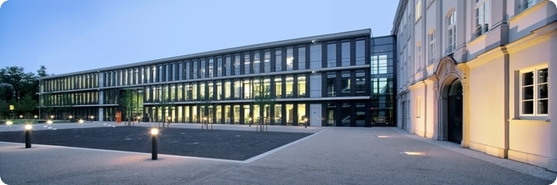
\includegraphics[width=0.6\textwidth]{./images/hochschule.jpg}
  %\end{center}
  %\vspace{-5pt}
  %\caption[Hochschule Augsburg]{Hochschule Augsburg \cite{HSA.2013}} % %Eckige Klammer (optional): Caption-Text in Abbildungsverzeichnis
  %\label{fig:hochschule}
  %\vspace{-5pt}
%\end{figure}

\subsection{Can Message Frame}
\label{subsec:can_bus_controller:can_frame}

In der Sprache des CAN-Standards werden alle Nachrichten als Frames bezeichnet; es gibt Daten-Frames, Remote-Frames, Error-Frames und Overload-Frames. Die an den CAN-Bus gesendeten Informationen müssen definierten Frame-Formaten von unterschiedlicher, aber begrenzter Länge entsprechen.
CAN verfügt über vier verschiedene Arten von Message Frames:

\begin{itemize}
	\item \textbf{Data Frame (Sendet Daten)}: Die Daten werden von einem Sendeknoten zu einem oder mehreren Empfangsknoten übertragen.
	\item \textbf{Remote Frame (Fordert Daten an)}: Jeder Knoten kann Daten von einem Quellknoten anfordern. Auf einen Remote-Frame folgt somit ein Daten-Frame, der die angeforderten Daten enthält
	\item \textbf{Error Frame (Meldet einen Fehlerzustand)}: Jeder Busteilnehmer, egal ob Sender oder Empfänger, kann zu jeder Zeit während einer Daten- oder Remote-Frame-Übertragung einen Fehlerzustand melden.
	\item \textbf{Overload-Frame  (Meldet Knotenüberlastung)}: Ein Knoten kann zwischen zwei Daten- oder Remote-Frames eine Verzögerung anfordern, das heißt, dass der Overload-Frame nur zwischen Daten- oder Remote-Frame-Übertragungen auftreten kann.
\end{itemize}

Im Nachfolgenden gegen wir auf der Architektur von den jeweiligen CAN Frame Typen ein.
\subsubsection{Data Frame}
\begin{figure}[h]
	 \begin{center}
	  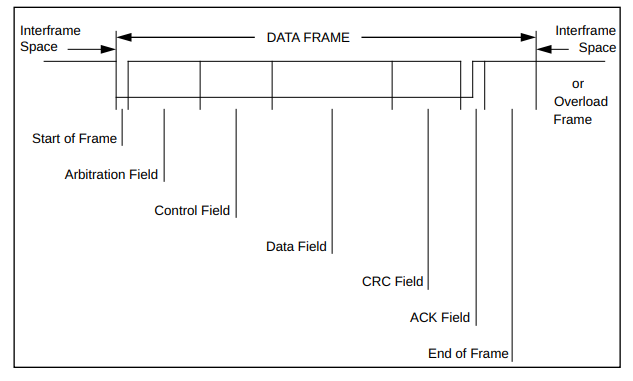
\includegraphics[width=1\textwidth]{./images/CAN-data-frame.jpg}
	\end{center}
	\vspace{-5pt}
	\caption[CAN-Data Frame Architektur]{CAN-Data Frame Architektur \cite{Bosch1991}[p.~12]} % Eckige Klammer (optional): Caption-Text in Abbildungsverzeichnis
	\label{fig:can-data-frame}
	\vspace{-5pt}
	\end{figure}
Die Abbildung ~\ref{fig:can-data-frame} beschreibt die 7 Bestandteile, aus denen ein Data Frame besteht, namlich:
\begin{itemize}
	\item \textbf{SOF}(Start of Frame):  Zeigt den Beginn von Daten und Remote Frames an.
	\item \textbf{Arbitration Field}: der besteht auf
		\begin{itemize}
			\item Identifikator: Die Basis-ID besteht aus 11 Bits und die erweiterte ID aus 29 Bits.
			\item RTR(Remote Transmission Request)-Bit: Im Data Frame ist das RTR-Bit "0". Im RTR-Frame hingegen ist es "1".
		\end{itemize}
	\item \textbf{Control Field}: Dient zur Bestimmung der Datengröße und der Länge der Nachrichten-ID. der besteht auf 6 Bits.
		\begin{itemize}
			\item IDE ( Identifikator-Erweiterung): Dieses Bit bestimmt den Identifikator als Basis-ID oder Erweiterte ID.
			\item R0,R1: reservierte Bits.
			\item DLD (Data Length Code): Er wird zur Bestimmung der Datenlänge verwendet.
		\end{itemize}
	\item \textbf{Data Field}: bis zu 8 Byte Datenfeld.
	\item \textbf{CRC-Field (Cyclic Redundancy Check)}: zur Überprüfung der Datenkorrektur.
	\item \textbf{ACK Field (Acknowledgement Field)}: um zu bestimmen, ob die Nachricht empfangen wurde oder nicht. Bei Empfang von Daten wird dieses Bit auf High gezogen.
	\item \textbf{EOF (End of Frame)}: Zeigt das Ende von Daten- und Remote-Frames an.
\end{itemize}

\subsubsection{Remote Frame}
\begin{figure}[h]
	\begin{center}
		\includegraphics[width=1\textwidth]{./images/CAN-remote-frame.jpg}
	\end{center}
	\vspace{-5pt}
	\caption[CAN-Remote Frame Architektur]{CAN-Remote Frame Architektur \cite{Bosch1991}[p.~17]} % Eckige Klammer (optional): Caption-Text in Abbildungsverzeichnis
	\label{fig:can-remote-frame}
	\vspace{-5pt}
\end{figure}
 Die Abbildung ~\ref{fig:can-remote-frame} beschreibt die Bestandtele einem Remote-Frame. Data-Frame und Remote-Frame sind sich beide sehr ähnlich. Im Prinzip ist der Remote Frame ein Data Frame ohne das Datenfeld. Dieser besteht in der Regel aus den gleichen Bestandteilen wie der Data Frame.
 
 \subsubsection{Error Frame}
 
 Abbildung ~\ref{fig:can-error-frame} zeigt die Struktur der Error Frame an. Der Error Frame besteht aus zwei Teilen:
 \begin{itemize}
 	\item Error Flag: stellt ein Knoten einen Fehlerzustand fest, erzeugt er bis zu 12 Bits "0" für das Fehlerflag.
 	\item Error Delimiter: 8 Bits "1" beenden den Error Frame.
 \end{itemize}
 
 \begin{figure}[h]
 	\begin{center}
 	  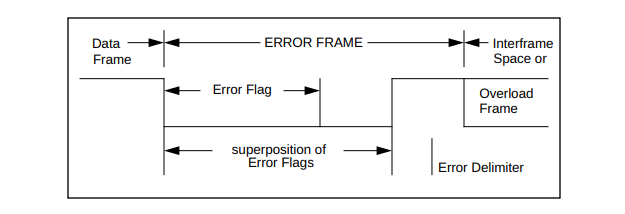
\includegraphics[width=1\textwidth]{./images/Can-error-frame.jpg}
 	\end{center}
 	\vspace{-5pt}
 	\caption[Can-Error-Frame]{Can-Error-Frame \cite{Bosch1991}[p.~18]} % Eckige Klammer (optional): Caption-Text in Abbildungsverzeichnis
 	\label{fig:can-error-frame}
 	\vspace{-5pt}
 \end{figure}

\subsubsection{Overload Frame}
 Abbildung ~\ref{fig:can-overload-frame} ist der Überlastrahmen. Er wird von dem Empfängerknoten erzeugt, um mehr Verzögerung zwischen den Datenrahmen zu erzwingen.

\begin{figure}[h]
	\begin{center}
		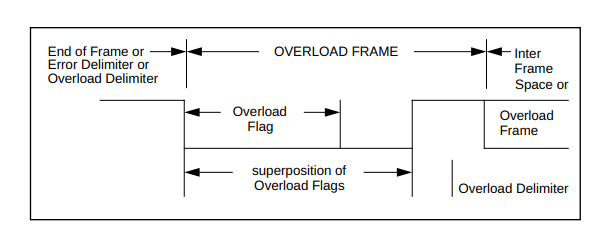
\includegraphics[width=1\textwidth]{./images/Can-overload-frame.jpg}
	\end{center}
	\vspace{-5pt}
	\caption[Can-Overload-Frame]{Can-Overload-Frame \cite{Bosch1991}[p.~19]} % Eckige Klammer (optional): Caption-Text in Abbildungsverzeichnis
	\label{fig:can-overload-frame}
	\vspace{-5pt}
\end{figure}



%\paragraph*{Beispiel}-----------Paragraph erstellen
%------------------- wrapfigure einfügen----------------------
%\begin{wrapfigure}{r}{0.45\textwidth}
 % \vspace{-20pt}
  %\begin{center}
  %  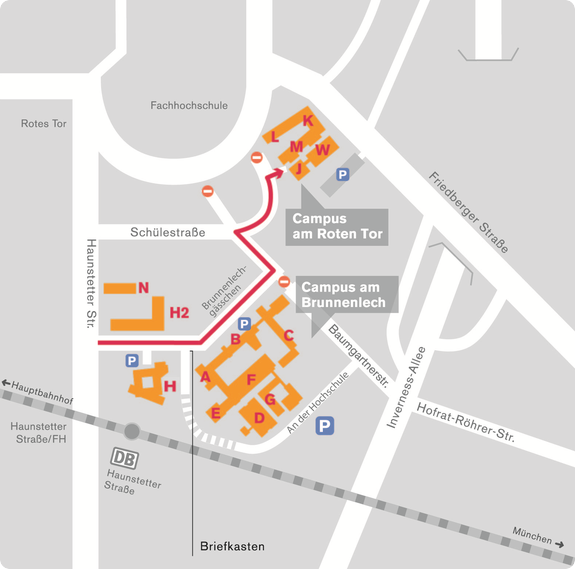
\includegraphics[width=0.45\textwidth]{./images/standort_rotes_tor_anfahrt_klm_bau.png}
  %\end{center}
  %\vspace{-20pt}
  %\caption[Standort Rotes Tor]{Standort Rotes Tor \cite{HSA.2013}}
  %\label{fig:standort_rotes_tor_anfahrt_klm_bau}
  %\vspace{-10pt}
%\end{wrapfigure}

\subsection{Can Physical Layer}
\label{subsec:can_bus_controller:can_physical_layer}
Der CAN FD Protokoll, der während dieser Arbeit verwendet wird, ist in ISO 1189-1:2015 definiert. Dieses Protokoll beschreibt nicht die mechanischen, Drähte, und Anschlüsse, aber fordert allerdings, dass die Drähte und Anschlüsse den elektrischen Spezifikationen entsprechen müssen. 
\begin{figure}[h]
	\begin{center}
		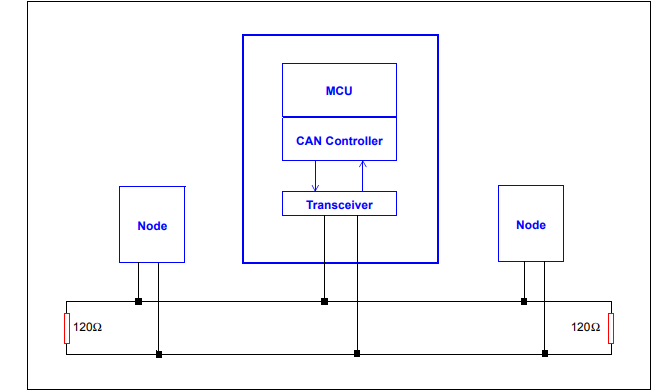
\includegraphics[width=1\textwidth]{./images/Can-connexion.jpg}
	\end{center}
	\vspace{-5pt}
	\caption[Can-Bus Connexion]{Can-Bus Connexion \cite{Richards2002}[p.~2]} % Eckige Klammer (optional): Caption-Text in Abbildungsverzeichnis
	\label{fig:can-bus-connexion}
	\vspace{-5pt}
\end{figure}
Abbildung ~\ref{fig:can-bus-connexion} zeigt eine CAN-Verbindung mit zwei CAN-Node gemäß der ISO-11898-1 CAN-Spezifikation. CAN High(CAN_H) und CAN Low(CAN_L) verlangen zwei 120\si{\ohm}-Abschlusswiderstände. Der Transceiver wandelt die von CAN-Knoten kommenden CAN-Signale in ein digitales Rx- und Tx-Signal für den Node Controller um.
Des Weiteren handelt es sich bei CAN_H und CAN_L um Differenzsignale. wie auf der Abbildung  ~\ref{fig:can-h:can-l}  zu sehen ist, wenn die zwei Signale bei 2,5 V liegen, ist dies ein rezessives Signal, also eine logische 0. Wenn CAN_H auf 3,5 V und CAN_L auf auf 1,5 V, dann handelt es sich um ein dominantes Signal, also eine logische 1. 
\begin{figure}[h]
	\begin{center}
		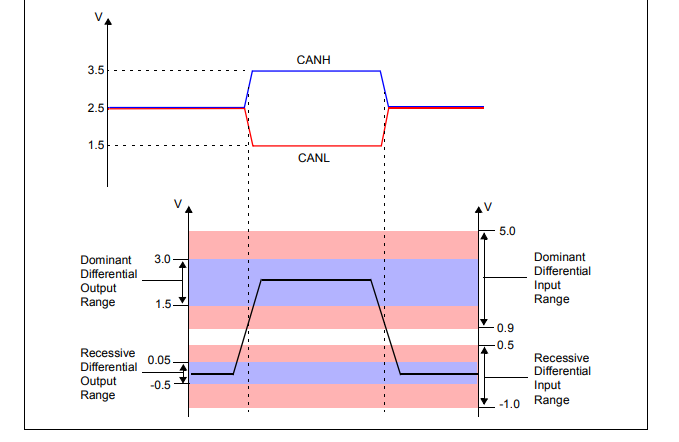
\includegraphics[width=1\textwidth]{./images/can-high-low.jpg}
	\end{center}
	\vspace{-5pt}
	\caption[CAN_H and CAN_L]{CAN_H and CAN_L \cite{Richards2002}[p.~3]} % Eckige Klammer (optional): Caption-Text in Abbildungsverzeichnis
	\label{fig:can-h:can-l}
	\vspace{-5pt}
\end{figure}
\section{SPI Interface}
\label{sec:SPI:Interface}

Die \Fachbegriff{Serial Peripheral Interface} (SPI) ist eine der am häufigsten verwendeten Schnittstellen zwischen Mikrocontrollern und Peripherie-ICs wie Sensoren, ADCs, DACs, Schieberegistern, SRAM und anderen. 
Die Schnittstelle SPI ist eine synchrone, auf Voll-Duplex basierte Master-Slave-Schnittstelle. Die Daten vom Master oder Slave werden mit der aufsteigenden oder abfallenden Taktflanke synchronisiert. Dabei können sowohl Master als auch Slave gleichzeitig Daten übertragen. \\
Das SPI arbeitet aber nach dem Single-Master-Prinzip. Das bedeutet, dass ein zentrales Gerät die gesamte Kommunikation mit den Slaves initiiert. Der Master sendet Daten auf der MOSI-Signalleitung und empfängt Daten auf der MISO-Signalleitung, so dass der Busmaster gleichzeitig Daten senden und empfangen kann. wie auf dem Bild A der Abbildung ~\ref{fig:spi:bus} zu sehen ist. Alle Datenübertragungen müssen zwischen dem Bus-Master und den Slaves stattfinden. Datenübertragungen die direkt zwischen zwei Slave-Geräten stattfinden  sind nicht erlaubt. 

\begin{figure}[h]
	\begin{center}
		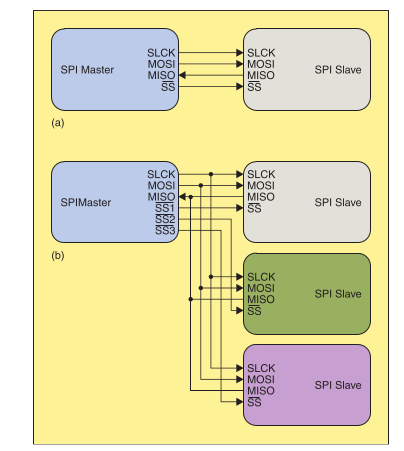
\includegraphics[width=0.8\textwidth]{./images/spi-bus.jpg}
	\end{center}
	\vspace{-5pt}
	\caption[SPI Bus]{SPI Bus \cite{Leens2009}[p.~9]} % Eckige Klammer (optional): Caption-Text in Abbildungsverzeichnis
	\label{fig:spi:bus}
	\vspace{-5pt}
\end{figure}
Möchte der SPI-Master Daten an einen Slave senden und/oder von ihm Informationen anfordern, dann wählt er einen Slave aus, und zwar durch Ziehen der entsprechenden SS-Leitung nach unten, während er das Taktsignal mit einer für den Master und den Slave nutzbaren Taktfrequenz aktiviert.
SPI ist eine Protokoll mit vier Signalleitungen, wie auf \cite{Leens2009}[p.~9] zu lesen ist.
\begin{itemize}
	\item \textbf{Ein Clock-Signal (SCLK)}, welches vom Bus-Master an alle Slaves gesendet wird; alle SPI-Signale sind mit diesem Clock-Signal synchronisiert.
	\item \textbf{Der Slave Select Signal}: der zur Auswahl des Slaves dient, mit dem der Master kommuniziert.
	\item \textbf{Eine Datenleitung vom Master zu den Slaves}, bezeichnet als Master Out-Slave In (MOSI).
	\item \textbf{Eine Datenleitung von den Slaves zum Master}, bezeichnet als Master In-Slave Out (MISO).
\end{itemize}
%\begin{minipage}{\textwidth}
 % \captionof{lstlisting}[Hello World]{Hello World \cite{coder.2009}} % Eckige Klammer (optional): Caption-Text in Listingsverzeichnis
  %\vspace{-3pt}
  %\begin{lstlisting}[language=java,label=lst:HelloWorld]
%public class HelloWorld
%{
%  public static void main(String[] args)
 % {
  %  System.out.println("HelloWorld");
  %}
%}
%  \end{lstlisting}
%\end{minipage}
\section{Embedded Linux}
\label{cha:ver:sec:Embedded_Linux}



\section{Komponente des Embedded Linux Betriebssystems für ARM Prozessoren}
\label{cha:tech_grund:sec:Komponente_eines_Emb_Lin_Sys}
In diesem Abschnitt möchte ich auf die wesentlichen Komponenten von eingebetteten Linux-Betriebssystems im Detail eingehen. Im Anschluss daran wird der typische Boot-Prozess solcher Systeme beschrieben.
Ein auf Linux basierendes Betriebssystem wird in Form einer Linux-Distribution angeboten. Es handelt sich dabei um eine Sammlung von Softwarepaketen, Bibliotheken und Dienstprogrammen zusammen mit einer eigenen Linux-Kernel-Variante, die für eine bestimmte Prozessorarchitektur angepasst oder verändert wird. 
Zum Booten eines Linux-Betriebssystems auf einem ARM-Prozessor werden die folgenden Komponenten benötigt:

\begin{itemize}
	\item \textbf{der Bootloader} 
	\item \textbf{Der Gerätebaum(Device-tree)}:
	\item \textbf{Der Linux Kernel}
	\item \textbf{Root filesystem}: beinhaltet die Bibliotheken und Programme, die ausgeführt werden, sobald der Kernel seine Initialisierung abgeschlossen hat.
	\item \textbf{Der \grqq Init\grqq\ Prozess}:
\end{itemize}

\subsection{Der Bootloader}
\cite{Dervis2013}Der Bootloader ist die Software, die beim Einschalten des Systems ausgeführt wird und für das Laden eines Betriebssystems für die Hardware verantwortlich ist. Beim Einschalten des Rechners, auf denen Linux als Betriebssystem installiert ist, wird nach der ersten Einrichtung der Bootloader, der für die Initialisierung der Hardware-Peripherie und das Laden des Bitstreams im FPGA verantwortlich ist, in den Speicher geladen und der Code ausgeführt.\\
Der Bootloader muss zunächst von der Festplatte in den Prozessorspeicher geladen werden, bevor er ausgeführt werden kann. Beim Zynq UltraScale+MPSoC wird UBoot zum Laden des Linux-Kernels verwendet, und die Bootload-Phase ist hier in zwei Stufen unterteilt: die FSBL-Phase und die U-Boot-Phase

\subsection{Device-tree}
\begin{figure}[h]
	\begin{center}
		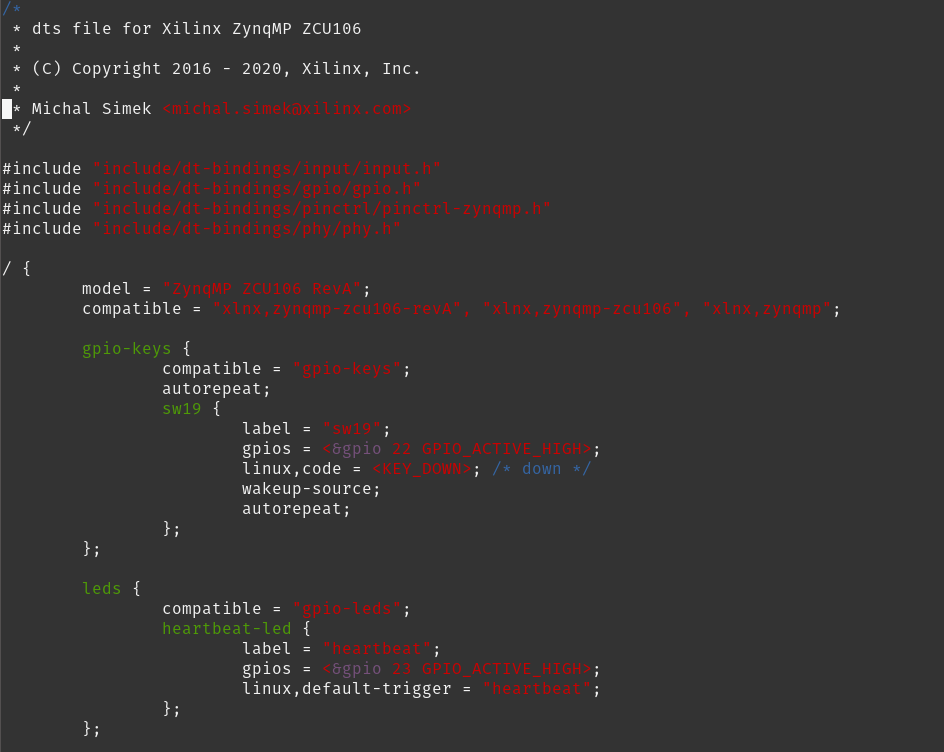
\includegraphics[width=1\textwidth]{./images/device-tree.jpg}
	\end{center}
	\vspace{-5pt}
	\caption[ZCU106-Gerätbaum gpio-keys and leds]{Ein Screenshot des ZCU106-Gerätebaums, der den Inhalt des gpio-keys und leds  auf dem Board zeigt} % Eckige Klammer (optional): Caption-Text in Abbildungsverzeichnis
	\label{fig:device:tree}
	\vspace{-5pt}
\end{figure}	
Die Abbildung ~\ref{fig:device:tree} zeigt Informationen zu den Schalter- und led-Knoten im Device Tree des Xilinx ZCU106 Boards. Hier wird z.B. angegeben, an welchem gpio-Pin der Schalter SW9 auf der Platine angeschlossen ist.\\
\cite{Dervis2013}Der Linux-Kernel benötigt Informationen über den Prozessor, auf dem er ausgeführt wird, die Peripheriegeräte, mit denen der Prozessor verbunden ist, ihre Schnittstellen zum Prozessor und ihre physikalischen Adressen. Der Kernel muss zur Initialisierung der Treiber und der mit diesen Peripheriegeräten verbundenen Dienste auch überprüfen, dass die Funktionen, die in seiner Konfiguration aktiviert wurden, tatsächlich von der Hardware unterstützt werden, die er steuert. Dabei kann es sich um Informationen über die Taktgeber und Register der Hardware oder über die mit der Hardware verbundenen Peripheriegeräte wie den externen Speicher, SPI handeln.\\

Der Zynq UltraScale+MPSoC verwendet daher den Device-Tree, um die Geräte- und Peripherie-Informationen wie physikalische Geräteadressen, E/A-Registeradressen, Speicheradressraum und Interrupt-Informationen während des Bootvorgangs an den Kernel weiterzugeben.\\
Der Gerätebaum wird im Textformat in einer Datei mit der Erweiterung \ ".dts"\ dargestellt. Hierbei handelt es sich um eine Quelltextdatei, die Informationen über Geräte und Verbindungsbusse beschreibt, die mit einer Computer-Hardware verbunden sind. Sie ist in Form von \ "Knoten"\ organisiert, deren Stammverzeichnis durch \grqq /\grqq\ dargestellt wird, genau wie im Linux-Stammdateisystem. Jeder Knoten hat einen Namen, der ein mit dem Prozessor verbundenes Gerät oder einen Bus darstellt, und der Knoten besteht aus Eigenschaften. Jeder übergeordnete Knoten für ein bestimmtes Peripheriegerät oder einen Bus kann \ "Kind"\ -Knoten für Geräte enthalten, die mit diesem Peripheriegerät oder Bus verbunden sind. Die Werte der Eigenschaften können Zeichenketten oder Listen von Zeichenketten sein, oder sie können leer sein, wenn das Vorhandensein oder Nichtvorhandensein des Wertes eine boolesche Logik an den Kernel übermittelt. Die Device-Tree-Quelldatei wird mit Hilfe des \ "dtc -Compilers"\ zu einem Device-Tree-Blob (.dtb) kompiliert.

\subsection{Der Linux Kernel}
Das ist das Herzstück des Systems, das die Systemressourcen und Schnittstelle zur Hardware verwaltet. Die Hauptfunktionen des Linux-Kernels sind die folgenden~\cite{linuxkernel.}:
\begin{itemize}
	\item Planung von Prozessen und Einrichten einer Umgebung für ihre Ausführung.
	\item  Zuteilung von Speicher an einen Prozess und Schutz des von einem Prozess verwendeten Speichers vor anderen Prozessen.
	\item \ Verwaltung der Kommunikation zwischen den Prozessen, um eine effiziente Ausführung der Prozesse zu gewährleisten
	\item Sicherstellung der Integrität des Systems, wenn das Computersystem mehrere Benutzer hat, die berechtigt sind, Änderungen am Root-Dateisystem und an Softwarepaketen vorzunehmen.	
	\item Verwalten der Computerressourcen und des Zugriffs auf diese Ressourcen
\end{itemize}

Nachdem der Bootloader den Gerätebaum und den Kernel in den DRAM des Prozessors geladen hat, teilt er dem Kernel die Adresse des Gerätebaums mit, bevor der Kernel mit der Ausführung beginnt. Der Kernel prüft dann der Reihe nach alle Hardware-Peripheriegeräte, Clock-Generator und Speicher, die vom FSBL initialisiert wurden, und aktiviert dann alle mit der zugrunde liegenden Hardware verbundenen Dienste und Funktionen, die in der Kernelkonfiguration aktiviert wurden. Sobald der Kernel mit diesen Aufgaben fertig ist, hängt er das Root-Dateisystem ein und führt den "init"-Prozess aus, der es dem Benutzer ermöglicht, in den Benutzerraum einzutreten.

\subsection{Das Linux Root files System (Rootfs)}

Das Linux-Root-Dateisystem [\cite{Dervis2013}] enthält alle binären ausführbaren Dateien, Geräteinformationen, Prozessprotokolle, Softwarepakete und Bibliotheken, die vom Benutzer in seinem Benutzerbereich benötigt werden, um das Linux-Betriebssystem effizient zu nutzen. Das Dateisystem auf der Festplatte ist in Verzeichnissen organisiert. Das Root-Dateisystem wird in das Verzeichnis\grqq /\grqq\ des Dateisystems eingehängt, welches die Spitze der Hierarchie des Root-Dateisystems markiert.

\subsection{Der Init Prozess}

Der "init"-Prozess [\cite{Dervis2013}] wird als erster Prozess im Benutzerbereich vom Kernel initiiert und ist für die Initialisierung der Systemverwaltungsdienste zuständig, bevor die Benutzer sich anmelden können. Alle Software-Dienste, die im Root-Dateisystem installiert und im Benutzerraum aktiviert wurden, werden vom "init"-Prozess ausgeführt, bevor sich die Benutzer sich am System anmelden

Als Nächstes wird den Boot-Prozess bei Systemen, die auf Zynq UltraScale+ MPSoCs basiert sind, erläutert, da dies genau die Plattform ist, die wir für unsere Arbeit verwenden werden.

\subsection{Der Zynq UltraScale+MPSoC Boot-Prozess}

Zum Booten von Linux auf dem Zynq UltraScale+MPSoC muss das Boot-Image (BOOT.BIN) auf dem Boot-Medium entsprechend dem vom Benutzer gewählten Boot-Modus vorhanden sein [\cite{Xilinx2017}[p.~14]]. Das ZCU106 Board unterstützt das Booten über JTAG, Quad-SPI Flash, SD Card und NAND Flash Drive. In dieser Arbeit booten wir Linux von der SD-Karte[\cite{Xilinx2020}[p.~61]], daher muss die Datei BOOT.BIN auf der FAT32-Partition der SD-Karte vorhanden sein. Die BOOT.BIN-Datei wurde so konfiguriert, dass sie die Platform Management Unit Firmware (PMUFW), die FSBL und die ausführbaren U-Boot-Dateien beinhaltet, welche die empfohlene Konfiguration für den Zynq UltraScale+ ist. Die BOOT.BIN enthält in dieser Arbeit auch den FPGA-Bitstream zur Programmierung der programmierbaren Logik (PL). Für ein vollständiges Booten über eine SD-Karte sollten das Kernel-Image (Image) und der Device-Tree-Blob ("Projektname.dtb") ebenfalls auf der FAT32-Partition vorhanden sein. Das Root-Dateisystem muss auf der EXT4-Partition der SD-Karte vorhanden sein.\\
Der Bootvorgang von Linux auf dem Xilinx Zynq UltraScale+MPSoC lässt sich in vier Phasen unterteilen

\begin{itemize}
	\item Die Boot-Setup-Phase
	\item Die Bootloader-Phase
	\item Die Kernel-Boot-Phase
	\item und Die \grqq init\grqq-Phase
\end{itemize}

\subsubsection{Die Boot-Setup-Phase}

Die Platform Management Unit (PMU) und die Configuration Security Unit (CSU) sind für das Einrichten des Zynq UltraScale+ MPSoC verantwortlich, bevor Linux auf dem PS gebootet werden kann . Die Boot-Setup-Phase besteht aus drei Phasen, die wie folgt unterteilt werden können[\cite{XilinxInc.2019}[p.~27]]:
\begin{itemize}
	\item \textbf{Pre-configuration stage (Oder Vor-Konfigurationsphase)}: Dieser Phase wird von der PMU angesteuert, die den PMU-ROM-Code(PBR). Nachdem der PBR-Code ausgeführt wurde, übergibt er die Systemkontrolle an die Configuration Security Unit (CSU). Die wichtigsten Schritte der Vor-Konfigurationsphase sind im Folgenden aufgeführt[\cite{XilinxInc.2019}[p.~57]]:
	\begin{itemize}
		\item Initialisieren des Systemmonitors
		\item Initialisierung der Phase Locked Loops (PLL) für Takte
		\item Leeren des PMU-RAMs.
		\item Initialisieren Sie des Dynamic Random Access Memory (DRAM).
		\item Freigabe der CSU oder Eintritt in den Fehlerzustand.
	\end{itemize}
	\item \textbf{Configuration stage oder (Konfiguration der Phase)}:Diese Phase übernimmt das Laden des First-Stage-Bootloader-Codes (FSBL) für den PS in das On-Chip-RAM (OCM), und zwar sowohl im sicheren als auch im unsicheren Boot-Modus. Während des Bootvorgangs lädt die CSU auch die PMU-Benutzerfirmware (PMU FW) in das PMU-RAM, um in Verbindung mit dem PMU-ROM Plattform-Management-Dienste bereitzustellen.
	\item \textbf{Post-configuration stage oder (Post-Konfigurationsphase)}: Nach dem Start der FSBL-Ausführung geht der CSU-ROM-Code in die Post-Konfigurationsphase über, die für die Reaktion auf Systemmanipulationen verantwortlich ist
\end{itemize}

\subsubsection{Die Bootloader-Phase}
\textbf{\normalsize First Stage Bootloader (FSBL)}\\
Die FSBL ist der sekundäre Programmlader in der Terminologie des generischen ARM-Prozessor-Boot-Prozesses. Der FSBL führt die folgenden Aufgaben aus. FSBL führt die folgenden Aufgaben aus[\cite{XilinxInc.2019}]
\begin{itemize}
	\item Suchen in der FAT32-Bootpartition der SD-Karte nach dem PL-Bitstream und dem second stage Bootloader (das U-boot).
	\item Initialisierung der PS-Hardware, der E/A-Geräte, des Speichers und der Takte entsprechend der Konfiguration, die durch das in der Xilinx Vivado Design Suite spezifizierte Hardware-Design definiert ist
	\item Programmieren des PL mit dem FPGA-Bitstream
	\item Laden der ARM Trusted Firmware (ATF) und das U-Boot in den APU-Prozessorspeicher.
\end{itemize}

\textbf{\normalsize Das U-boot}\\
Wenn der Prozessor eingeschaltet wird, enthält der Prozessorspeicher kein Betriebssystem, sodass ein Bootloader erforderlich ist, um den Linux-Kernel und den Gerätebaum aus dem Speicher in den Prozessorspeicher zu laden, diese Aufgabe wird also vom U-boot Übernomen. Der U-Boot ist der Second Stage Bootloader (SSBL) für den Xilinx Zynq UltraScale+ MPSoC oder der Tertiary Program Loader (TPL) in der Terminologie des generischen ARM-Bootprozesses.  U-Boot kann den Kernel und den Device-Tree über das Netzwerk mittels Ethernet, über JTAG, von der SD-Karte, Quad-SPI-Flash und vom NAND-Flash-Laufwerk laden.

Die Abbildung ~\ref{fig:boot:process} Es zeigt die Rolle der verschiedenen Einheiten des Zynq UltraScale+MPSoC beim Booten des Linux-Betriebssystems auf der Hardware. Man sieht, dass die PMU die CSU freigibt, die wiederum die FSBL lädt. Die FSBL lädt dann das ATF und das U-Boot. Das U-Boot ist dann für das Booten von Linux auf der Hardware verantwortlich.

\begin{figure}[h]
	\begin{center}
		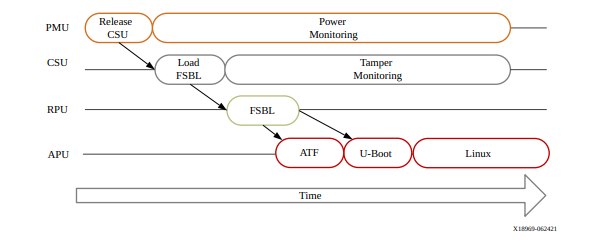
\includegraphics[width=1.1\textwidth]{./images/boot-flow.jpg}
	\end{center}
	\vspace{-5pt}
	\caption[der Bootvorgang bei zynq+MPSoCs]{Überblick über den Bootvorgang \cite{XilinxInc.2019}[p.~58]} % Eckige Klammer (optional): Caption-Text in Abbildungsverzeichnis
	\label{fig:boot:process}
	\vspace{-5pt}
\end{figure}


\subsubsection{Der Boot Flow}

Der Zynq UltraScale+ MPSoC kann in zwei Modi gebootet werden: im sicheren und im unsicheren Modus. Diese werden im Folgenden beschrieben[\cite{XilinxInc.2019}[p.~58]]

\textbf{\normalsize Nicht gesicherter Bootvorgang}\\
In diesem Boot-Modus gibt die PMU die CSU frei und wechselt in den Servicemodus, in dem sie die Plattform überwacht. Die CSU lädt die FSBL in den On-Chip-Speicher (OCM) der APU und die PMUFW in das RAM der PMU. Die PMUFW wird parallel zur Ausführung der FSBL ausgeführt und läuft, bis Linux auf dem Zynq UltraScale+ MPSoC gebootet ist. Der FSBL initialisiert die Peripheriegeräte, E/A-Geräte, den Speicher und die Takte und übergibt sie an den ATF, der sie dann an das U-Boot weitergibt. Das U-Boot lädt dann den Linux-Kernel in das APU-Prozessor-Memo

\textbf{Sicherer Bootvorgang}\\

Der sichere Bootvorgang unterscheidet sich vom unsicheren Bootvorgang nur durch einige zusätzliche Authentifizierungs- und Entschlüsselungsschritte, die von der CSU ausgeführt werden. Beim sicheren Bootvorgang gibt die PMU den Reset der Configuration Security Unit (CSU) frei und geht in den PMU-Servermodus über, in dem sie die Stromversorgung überwacht. Nachdem die PMU das Zurücksetzen der CSU aufgehoben hat, prüft die CSU, ob eine Authentifizierung durch die FSBL oder die Benutzeranwendung erforderlich ist 

\subsection{Die Kernel-Boot-Phase}
Das U-Boot sorgt für das Laden des Kernel-Images und des Gerätebaums in den Speicher des APU-Prozessors und die Übergabe der Kontrolle an den Kernel. Der Kernel erhält auch die Adresse des Gerätebaums, der den Kernel über die Hardware-Peripherie, E/A-Geräte, Speicher und Taktgeber informiert. Basierend auf diesen Informationen startet der Kernel den Bootvorgang und aktiviert die Treiber und Dienste, für die der Kernel konfiguriert wurde. Nachdem der Kernel gebootet hat, mountet er das Root-Dateisystem entsprechend den an den Kernel übergebenen Boot-Argumenten. Je nach dem an den Kernel übergebenen Boot-Argument hängt der Kernel das Root-Dateisystem über NFS oder von der SD-Karte oder einem anderen permanenten Speicherort ein.

\subsection{Die init-Phase}

Nach Einhängen des Root-Dateisystems sucht der Kernel nach der ausführbaren Datei des für die Linux-Distribution angegebenen init-Prozesses. Sobald der Kernel den init-Prozess gefunden hat, führt er ihn aus und übergibt die Kontrolle an den init-Prozess. Der init-Prozess aktiviert dann alle Systemverwaltungs- und andere Hintergrunddienste, die im Root-Dateisystem installiert und im Benutzerbereich aktiviert wurden. Nach der Aktivierung dieser Dienste startet der init-Prozess den Benutzeranmeldungsprozess, der es dem Benutzer ermöglicht, den Benutzerraum zu betreten\\
Alle bisher genannten Linux-Komponenten, ob der Bootloader, der Kernel oder das Root-Dateisystem können mit einem Build-System wie dem Yocto-Projekt erstellt werden. Da unser FPGA aber einen MPsoc enthält, der einen Bootloader, ATF-Firmware, pmufw, den Bitstream und u-boot benötigt, ist ein Build System zu verwenden, das automatisch alle diese Komponenten erzeugen kann.. Hierfür ist Petalinux am besten geeignet. Im nächsten Abschnitt werde ich das Petalinux Build System vorstellen. 



\section{Petalinux Tool Flow}
\label{sec:Petalinux_Toolflow}
PetaLinux ist ein Embedded Linux Software Development Kit (SDK), das auf FPGA-basierte System-on-a-Chip (SoC)-Designs abzielt[\cite{Xilinx2020}]. Es setzt sich praktisch auf Yocto auf, so wird das Root-Dateisystem unter Verwendung von Yocto erstellt. Unter PetaLinux versteht man eine Reihe von High-Level-Befehlen, die auf der Yocto-Linux-Distribution aufbauen. Die PetaLinux-Werkzeuge können zur Anpassung, Erstellung und Bereitstellung von Embedded Linux-Lösungen/Linux-Images für Xilinx-Prozessorsysteme verwendet werden. 
Ein wesentlicher Vorteil von petalinux ist, dass es eine Reihe von vereinfachten Befehlen enthält, die für das Booten und die Integration von HW- und SW-Projekten sehr nützlich sind. In Abbildung ~\ref{fig:petalinux:tool:flow} sieht man einen Überblick über den PetaLinux-Werkzeugfluss auf oberster Ebene.
	
\begin{figure}[H]
	\begin{center}
		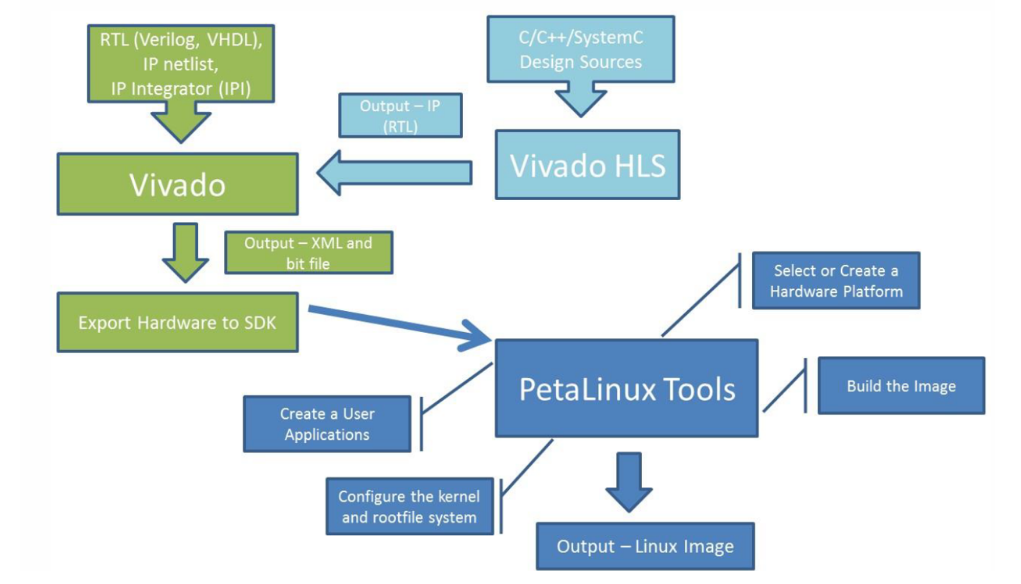
\includegraphics[width=1.1\textwidth]{./images/petalinux-toolflow.jpg}
	\end{center}
	\vspace{-5pt}
	\caption[PetaLinux-Werkzeugfluss]{Überblick über den PetaLinux-Werkzeugfluss [\cite{petailinuxtool}]} % Eckige Klammer (optional): Caption-Text in Abbildungsverzeichnis
	\label{fig:petalinux:tool:flow}
	\vspace{-5pt}
\end{figure}

Wie man in der Abbildung ~\ref{fig:petalinux:tool:flow} sehen kann, ist es möglich, mit Vivado erstellte Hardware-Designs in petalinux zu importieren, einige Anwendungen in petalinux einzubinden und ein Linux-Image zu erstellen.  

\subsection{Petalinux Installation}
Wie jedes Build-System benötigt petalinux viele Ressourcen auf Ihrem PC. Um die Kompilierzeit deutlich zu reduzieren, ist es daher sinnvoll, einen Computer mit folgenden Eigenschaften zu verwenden.\cite{Xilinx2020}

\begin{itemize}
	\item 8 GB RAM
	\item 2 GHz CPU-Takt oder gleichwertig
	\item 100 GB freier HDD-Platz
	\item Petalinux unterstützt nur auf Linux Kernel basierte Betriebssysteme. 
	\item PetaLinux-Tools erfordern, dass Ihr Host-System /bin/sh \textbf{bash} ist. Der folgende Befehl kann verwendet werden, um die Bash als Terminal einzurichten, wobei der Befehl als root ausgeführt werden muss. 
	\begin{lstlisting}[language=bash]
		$ sudo dpkg-reconfigure dash
	\end{lstlisting}
\end{itemize}
Bevor das Installationsprogramm ausgeführt wird, müssen eine Reihe von Abhängigkeiten installiert werden. Die folgenden Befehle installieren alle erforderlichen Pakete auf einmal:

\begin{lstlisting}[language=bash]
	$ sudo apt upgrade
	$ sudo apt install -y python3 tofrodos iproute2 gawk xvfb gcc git make net-tools libncurses5-dev tftpd zlib1g-dev ibssl-dev flex bison libselinux1 gnupg wget diffstat chrpath socat xterm autoconf libtool tar unzip texinfo zlib1g-dev gcc-multilib build-essential libsdl1.2-dev libglib2.0-dev screen pax gzip
\end{lstlisting}

 Einmal die vorherigen Voraussetzungen erfüllt, kann man also die Installationsdatei von Petalinux unter diesem Link \url{https://www.xilinx.com/support/download/index.html/content/xilinx/en/downloadNav/embedded-design-tools.html} herunterladen.\\ 
 mit dem \textbf{mkdir} Kommando in Linux kann man ein Petalinux Installation Ornder erstellen, in dem die Installationsdatei dann kopiert wird. mit dem -p Schalter kann den Ordner in einem spezifischen Ordner erstellen.\\
 
\begin{lstlisting}[language=bash]
 	$ mkdir -p /home/<user>/petalinux/<petalinux-version>
\end{lstlisting}

Mit den folgenden Befehlen kann man die Datei ausführbar machen und der Installationsprozess starten.
\begin{lstlisting}[language=bash]
 	$chmod 755 ./petalinux-v<petalinux-version>-final-installer.run
	$./petalinux-v<petalinux-version>-final-installer.run
\end{lstlisting}

\subsection{Wichtige Petalinux Kommando}
\label{sec:Petalinux_Toolflow:petalinux:kommando}
\begin{itemize}
	\item \textbf{petalinux-create}: Erstellt ein neue Petalinux Projekt. man kann dem Befehl verschiedenen Optionen zuweisen, 
	\begin{itemize}
		\item \textbf{\emph{type}}: definiert den Projekt Type
		
		\item \textbf{\emph{template}}: Bei der Erstellung des Projekts kann man eine Vorlage definieren. Für das Projekt wurde zynqMP verwendet.
		
		\item \textbf{\emph{srcuri}}: Hier wird der Pfad zu einem Board Support Package (BSP) angegeben, das zur Erstellung des Projekts verwendet wird. 
		
		\item \textbf{\emph{name}}: definiert der Name des Projekts. 
	\end{itemize}
	
	\item \textbf{petalinux-config}: dieser Befehl wird verwendet zur Initialisierung oder Aktualisierung der Hardwarekonfiguration des Projekts oder Konfiguration der Kernel- und/oder Dateisystemeinstellungen. Je nach Anwendung stehen hier auch uns eine Reihe von Konfiguration-Optionen zur Verfügung. Einige davon sind:
	\begin{itemize}
		\item \textbf{\emph{get-hw-description}}: Initialisiert den Petalinux-Projekt mit einem vom Vivado Hardware-description-file(HDF). PetaLinux verwendet HSI-Dienstprogramme, um Informationen über die Hardware aus dieser Datei zu extrahieren, sowie Informationen wie Intellectual property Cores (IP-Cores), Netze, Ports und Schnittstellen, die in anderen Tools wie dem Devicetree-Generator verwendet werden .
		
		\item \textbf{\emph{-c rootfs}}: Startet das Konfigurations-Menü des Root-Dateisystems.
		
		\item \textbf{\emph{-c kernel}}: Startet das Konfigurations-Menü des Kernel. 
	\end{itemize}
	
	\item \textbf{petalinux-build}: Das Tool Erstellt bestimmter Komponenten oder eines ganzen Linux-Systems für das PetaLinux-Projekt (einschließlich FSBL, uboot, Gerätebaum usw.). Genau so wie mit \textbf{\emph{petalinu-config}} Befehl, können auch Besonderheiten mit den Zeichen \textbf{-c} und \textbf{-x} festgelegt werden. 
	\begin{itemize}
		\item \textbf{\emph{-c oder --component}}: Baut die angegebene Komponente(kernel, u-boot, rootfs, device-tree ...). Es handelt sich hierbei um die Standard Komponente, die unterstützt werden. Es können aber auch eigenes Objekt erstellen werden (z. B. eigene Anwendung oder Modul). 
		\item \textbf{\emph{-x oder execute }}: Führt den angegebenen Build-Schritt aus. Es können alle Yocto-Tasks über diese Option übergeben werden(build, clean, cleansstate, distclean ...).
	\end{itemize}
	\item \textbf{petalinux-boot}: Das Werkzeug Bootet ein angegebenes Linux-Image entweder über JTAG auf die Hardware oder den QEMU-Softwareemulator.
	\begin{itemize}
		\item \textbf{\emph{-jtag}}: Die jtag-Tools sind sehr hilfreich, wenn man genau sehen möchte, wie der Boot-Vorgang im Einzelnen abläuft. 
	\end{itemize}
	\item \textbf{petalinux-package}: Das Werkzeug packt ein gebauter PetaLinux-Projekt in einem für die Bereitstellung geeigneten Format. je nach Zielpaketformat bietet es mehrere Arbeitsabläufe, deren Operationen abweichen. Für das Projekt verwenden wir  \textbf{\emph{	petalinux-package --boot}}, der hat die folgenden Optionen:
	\begin{itemize}
		\item \textbf{\emph{-format}}: Das zu erzeugendes Bilddateiformat(BIN, MCS,  DOWNLOAD.BIT)	
		
		\item \textbf{\emph{-fsbl}}: Damit definiert man den Pfad zum Firt Stage Bootloader(FSBL) .elf-Binäre Datei.
		
		\item \textbf{\emph{-fpga BITSTREAM}}: Den Pfad zur Bitstream-Datei.
		
		\item  \textbf{\emph{-force}}: Existierende Dateien auf der Festplatte überschreiben. 
	\end{itemize}
	\item \textbf{petalinux-devtool}: Das petalinux-devtool ist das letzte auf der Liste der petalinux-Tools, die ich beschreiben wollte und die ich für meine Arbeit benötigen werde. Das ist ein Dienstprogramm, das mit Hilfe des Yocto-Devtools Software erstellt, getestet und verpackt werden können. In den kommenden Abschnitte werde ich auf jeweilige Optionen, die ich verwendet habe eingehen. 
	
\end{itemize}

\subsection{Petalinux Projekt Strukture}
In diesem Abschnitt möchte ich über die Petalinux-Projektstruktur sprechen. Es ist wichtig, dies zu erwähnen, damit klar ist, wie und wo Komponenten, Module oder Software geändert werden können.

\begin{figure}[h]
	\begin{center}
		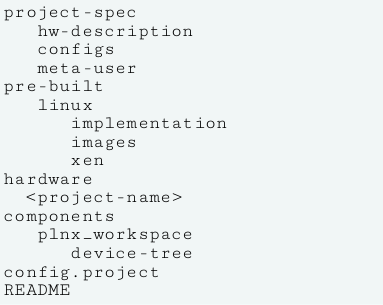
\includegraphics[width=0.7\textwidth]{./images/petalinux-projektstruktur.jpg}
	\end{center}
	\vspace{-5pt}
	\caption[petalinux Projektstruktur]{typische petalinux projektstruktur [\cite{petailinuxtool}]} % Eckige Klammer (optional): Caption-Text in Abbildungsverzeichnis
	\label{fig:petalinux:projektstruktur}
	\vspace{-5pt}
\end{figure}
In Abbildung ~\ref{fig:petalinux:projektstruktur} ist eine typische Petalinux Projektstruktur dargestellt. 

\begin{itemize}
	\item \textbf{project-spec}: In diesem Verzeichnis werden alle Änderungen an dem Projekt durchgeführt. Hier können z. B. neue Projekt Layers erstellen, den Gerätebaum(Device-tree) geändert oder sogar Rezepte für Software, die vom Kernel kompiliert werden soll, erstellt werden. 
	\item \textbf{pre-built}: Dieses Verzeichnis beinhaltet alle Board-spezifischen Design- und Konfigurationsdateien, vorgefertigte und getestete Hardware und Software-Images, die Sie auf dem Board direkt heruntergeladen werden können. Der Ordner ist jedoch nur sichtbar, wenn man das Projekt auf der Basis des für das Board spezifischen Board Support Package (BSP) erstellt hat. 
	\item \textbf{hardware}: 
	 
\end{itemize}

\clearpage

\chapter{Versuch Aufbau}
\label{cha:Versuch_Aufbau}
\section{Allgemein über das Projekt}
\label{cha:ver:sec:Allgemein_über_das_Projekt}
\section{Hardware Platform}
\label{cha:ver:sec:Hardware_Platform}

Aus Kostengründen wurde anstelle des FPGA-internen CAN-Controllers ein externer CAN-Controller verwendet. Und viel besser: Dieser CAN-Controller wurde im Unternehmen entwickelt.  Außerdem wurde das von Xilinx entwickelte Board ZCU106 verwendet, das auf dem Zynq Ultracale + MPSoC basiert. Das enthaltene ZU7EV-Gerät(Zynq Ultracale + MPSoC) integriert ein Quad-Core Arm Cortex-A53 Processing System (PS) und einen Dual-Core Arm Cortex-R5F Echtzeit-Prozessor. Das board verfügt auch über viele programmierbare digitale Komponenten, mit denen wiederum eine Vielzahl von Schaltungen realisiert werden können.Wie bereits erwähnt, ist das FPGA Bestandteil des ZCU106 Boards, das im nächsten Kapitel besprochen wird.

\subsection{Xilinx ZCU106 Evaluation Board}

Dieses Kapitel beschreibt die Xilinx ZCU106 Evaluation Board, insbesondere die Bereiche, die diese Plattform einzigartig machen. Dazu gehören die Zynq Ultrasale + MPSoC Architektur, das Processing System (PS) und die Programmable Logik (PL). Die Peripheriegeräte, die für die Interaktion mit dem CAN-Controller erforderlich sind, werden dabei erwähnt. Genauere Informationen dazu findet man im technischen Referenzhandbuch [\cite{XilinxInc.2019}] des Zynq-Plattforms. 

\begin{figure}[H]
	\begin{center}
		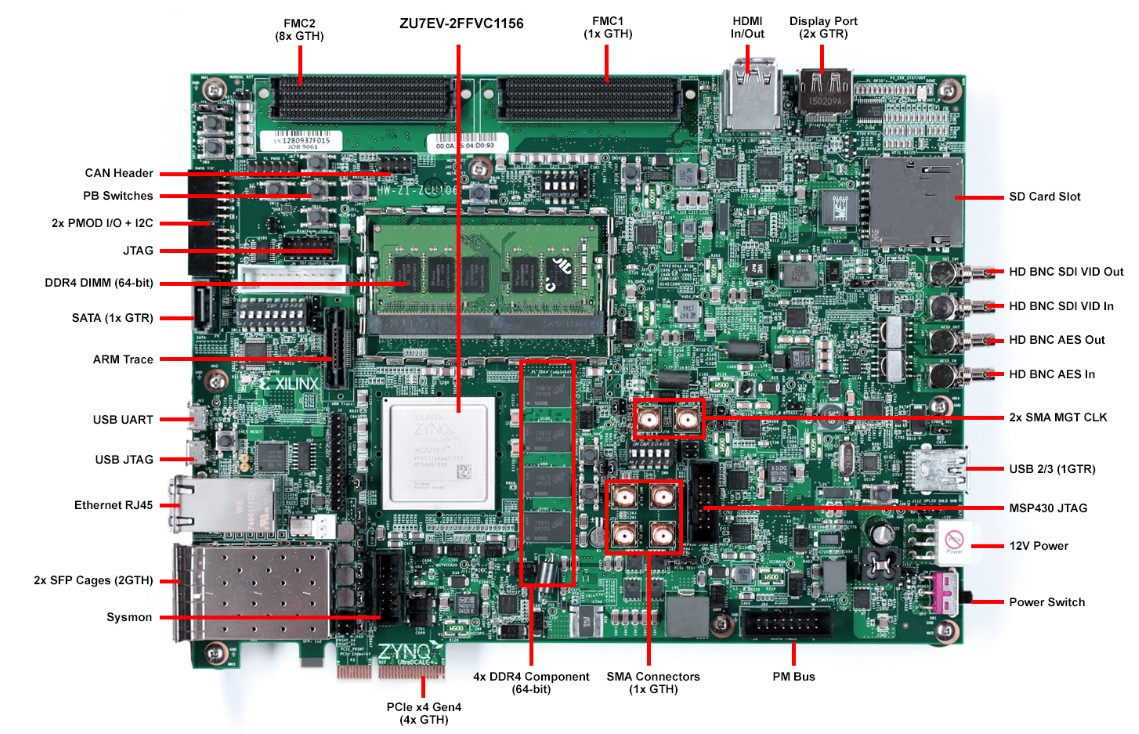
\includegraphics[width=1\textwidth]{./images/zcu106.jpg}
	\end{center}
	\vspace{-5pt}
	\caption[Xilinx ZCU102 Evaluation Board]{Xilinx ZCU102 Evaluation Board [\cite{zcuboard.}]}  %Eckige Klammer (optional): Caption-Text in Abbildungsverzeichnis
	\label{fig:zcu:board}
	\vspace{-5pt}
\end{figure}

%Es ist vorzusehen, dass das Betriebssystem auf mindestens einem der vier physischen Cortex-A53-Prozessoren des ZCU106 laufen wird, mit der Möglichkeit, Bar-Metal-Anwendungen auf anderen Prozessoren laufen zu lassen. 

%\begin{figure}[h]
%	\begin{center}
%		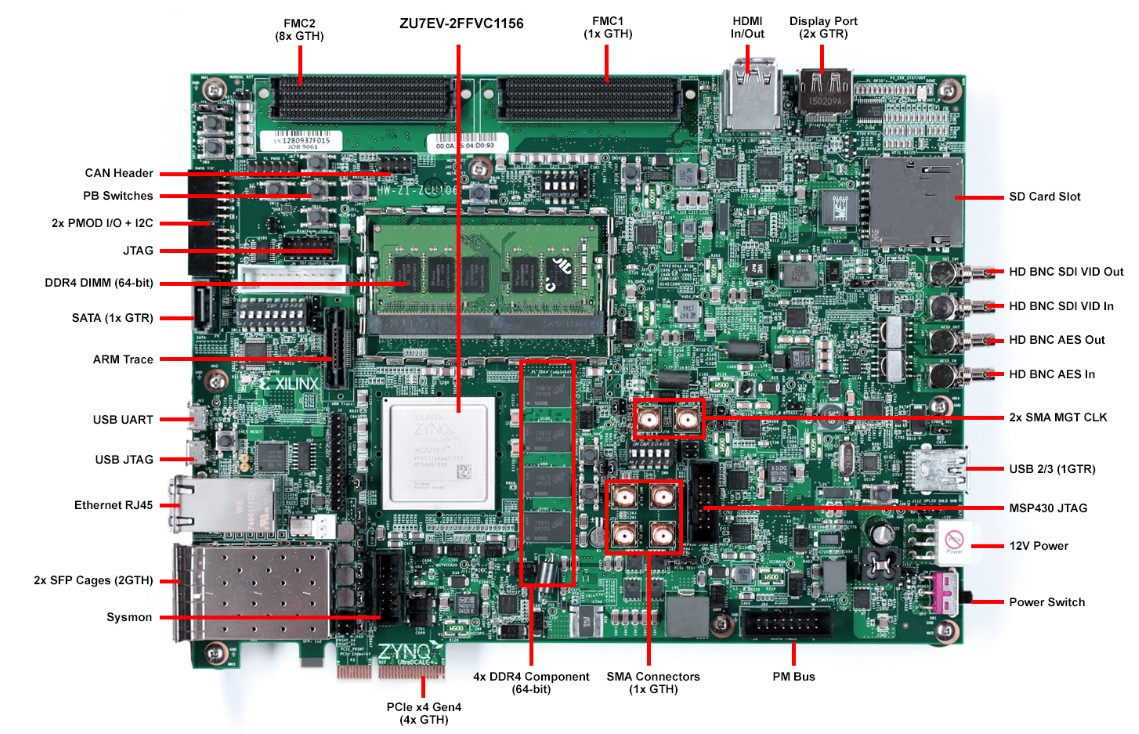
\includegraphics[width=0.98\textwidth]{./images/zcu106.jpg}
%	\end{center}
%	\vspace{-5pt}
%	\caption[Zynq UltraScale+ XCZU7EV-2FFVC1156 MPSoC]{Vortellung des Zynq UltraScale+ XCZU7EV-2FFVC1156 MPSoC} % Eckige Klammer (optional): Caption-Text in Abbildungsverzeichnis
%	\label{fig:zcu106}
%	\vspace{-5pt}
%\end{figure}

\subsubsection{Ultrasale + MPSoC Architektur}
Lassen wir uns, bevor wir uns mit der Zynq Ultrascale+ MPSoC-Architektur beschäftigen, ein wenig über die Zynq-Architektur im Allgemeinen sprechen. Es handelt sich bei Zynq um eine neue Generation von System-on-Chip (SoC), die eine CPU mit einem programmierbaren Logik-FPGA auf demselben Chip kombiniert.
FPGAs sind für ihre besondere Flexibilität beim Entwurf digitaler Schaltungen bekannt. Dennoch ist für viele Anwendungen der Entwurf einer riesigen Zustandsmaschine in Very High Speed Hardware Description Language (VHDL) oder Verilog nicht ausreichend. Stattdessen ziehen wir eine softwareprogrammierbare CPU-Architektur vor, die mit einfacheren FPGA-Blöcken zusammenarbeitet. Im Grunde genommen kann eine CPU jeden Algorithmus ausführen, so lange genug Speicher für ihre Bedürfnisse vorhanden ist. Softwarecode kann schnell geändert, neu kompiliert, gepatcht und debuggt werden. Die Rechenkapazität eines CPU-Kerns allein reicht jedoch oft nicht aus, um eine große Datenmenge zu verarbeiten. weshalb tendieren wir zu parallelen Architekturen, wie Multicore-CPUs, FPGAs und GPUs, um den Rechendurchsatz zu erhöhen.\\

Bislang gab es für jemanden, der eine CPU in Kombination mit einem FPGA benötigte, zwei Möglichkeiten: eine diskrete CPU und ein diskretes FPGA, die über einen Bus miteinander kommunizieren (was zu Bandbreitenbeschränkungen führte), oder eine Soft-Core-CPU. Diese wird direkt in den FPGA programmiert (z.B. 32-Bit Microblaze, 64-Bit Ultrascale, usw.). Die Entscheidung hängt von den Einschränkungen und Anforderungen der Anwendung ab, wie z. B. dem Systempreis, dem Stromverbrauch, der Komplexität und selbstverständlich der Leistung. Xilinx bietet mit der Zynq-Serie ein höheres Maß an Integration mit einer System-on-Chip-Hardcore-ARM-CPU, einem Xilinx-FPGA und Bussen für den effizienten Datentransfer zwischen beiden. Darüber hinaus umfassen die Zynq-Bausteine verschiedene Arten von Input/Output (I/O)-Controllern, Speicherschnittstellen und Hochgeschwindigkeits-Transceivern

\begin{figure}[H]
	\begin{center}
		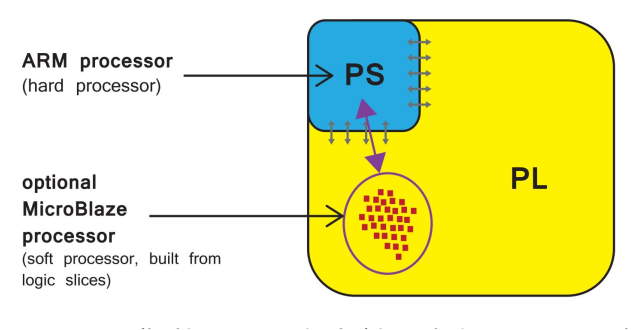
\includegraphics[width=1\textwidth]{./images/ps-pl.jpg}
	\end{center}
	\vspace{-5pt}
	\caption[Hard-(ARM Cortex-A9/Cortex-A53) und Soft-Prozessoren (MicroBlaze)]{Die Anordnung von Hard- (ARM Cortex-A9/Cortex-A53) und Soft-Prozessoren (MicroBlaze) auf einem Zynq/ZynqMP-Baustein [\cite{Crockett:2001018}]}  %Eckige Klammer (optional): Caption-Text in Abbildungsverzeichnis
	\label{fig:pl:ps}
	\vspace{-5pt}
\end{figure}


Die Abbildung ~\ref{fig:pl:ps} zeigt die Trennung zwischen dem festen Logik-Hardware-Prozessor und der programmierbaren Logik, die einen oder mehrere Soft-Prozessoren enthalten kann. 

\subsubsection{Allgemeine Ansicht des Zynq Ultrasale+ MPSoC}
Die Zynq Ultrascale+ MPSoC-Serie ist eine im Jahr 2015 von Xilinx eingeführte moderne SoC-Architektur [\cite{CNXSoftware}]. Abbildung ~\ref{fig:zynqmp:block:diagram} zeigt das Blockdiagramm des Zynq Ultrascale+ EG, der verfügt über mehrere Verarbeitungseinheiten wie die ARM Cortex A53 Application Processing Unit (APU) mit 4 Kernen, die Real-Time Processing Unit (RPU) und die Platform Management Unit (PMU). Die Abbildung zeigt die Schnittstelle zwischen dem Verarbeitungssystem (PS) und der programmierbaren Logik (PL). Die PL verfügt über mehrere Blöcke wie GPIO, Block-RAM und High-Connectivity-Block für die Implementierung von Designs zur Kommunikation mit Peripheriegeräten wie Ethernet oder SPI

\begin{figure}[H]
	\begin{center}
		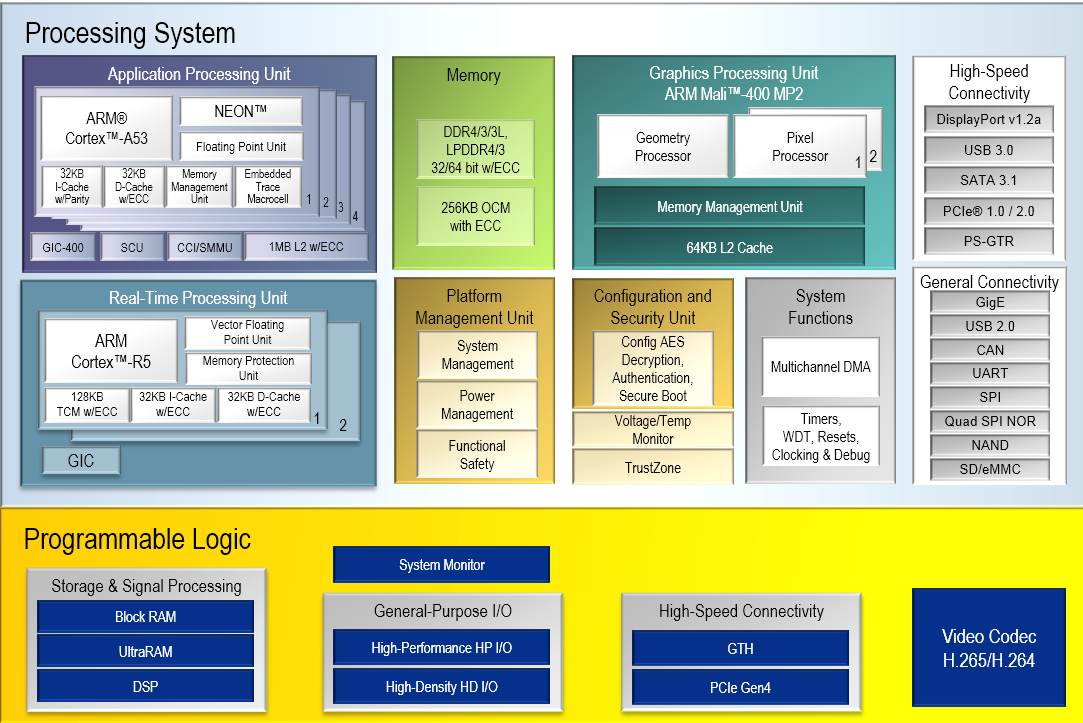
\includegraphics[width=1\textwidth]{./images/zynqmp-blockdiagramm.jpg}
	\end{center}
	\vspace{-5pt}
	\caption[Zynq UltraScale+ MPSoC EV Block Diagram]{Zynq UltraScale+ MPSoC EV Block Diagram [\cite{XilinxInc.}]} % Eckige Klammer (optional): Caption-Text in Abbildungsverzeichnis
	\label{fig:zynqmp:block:diagram}
	\vspace{-5pt}
\end{figure}

 Im Folgenden findet sich eine Liste der besonderen Komponente dieser Familie:
 \begin{itemize}
 	\item \textbf{APU}
 	\begin{itemize}
 		\item 64-bit Quad-core ARM Cortex-A53 1.5 GHz
 		\item NEON Media Processing Engine + Floating Point Unit (FPU)
 		\item Unterstützung für 32/64-Bit-Betriebsmodi
 		\item 32 KB Level-1 cache
 		\item 1 MB Level-2 cache
 	\end{itemize}
 	\item \textbf{RPU}
 	\begin{itemize}
 		\item 32-bit Dual-core ARM Cortex-R5  600 MHz
 	\end{itemize}
 	\item \textbf{graphics processing uni(GPU)}
 	\begin{itemize}
 		\item ARM Mali-400 MP2
 	\end{itemize}
 	\item \textbf{On-Chip Memory (OCM)}: 256KB
 	\item \textbf{Zwei 8-Channel Direct Memory Access (DMA) controllers}
 	\item \textbf{System Memory Management Unit (SMMU)}
 	\item \textbf{Platform Management Unit (PMU)}
 \end{itemize}
 
Der PS unterstützt auch viele Eingangs-/Ausgangsschnittstellen wie SRAM-Schnittstellen (SD, QSPI, NAND), GPIOs, UART usw.

\begin{figure}[H]
	\begin{center}
		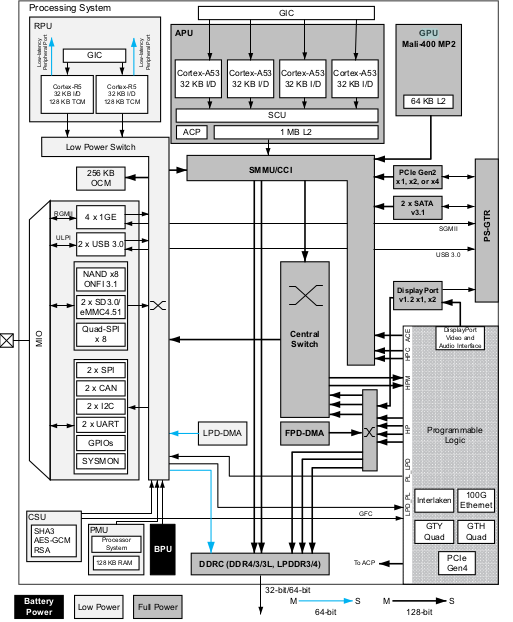
\includegraphics[width=1\textwidth]{./images/top-level_zynqmp.jpg}
	\end{center}
	\vspace{-5pt}
	\caption[Zynq UltraScale+ MPSoC Top-Level Blockdiagramm]{Zynq UltraScale+ MPSoC Top-Level Blockdiagramm [\cite{XilinxInc.2019}]} % Eckige Klammer (optional): Caption-Text in Abbildungsverzeichnis
	\label{fig:zynqmp:top:level}
	\vspace{-5pt}
\end{figure}

Im Top-Level-Blockdiagramm der Zynq MPSoC-Architektur ~\ref{fig:zynqmp:top:level} ist die Verbindung zwischen den verschiedenen Blöcken markiert. Da kann die verschiedenen Verarbeitungseinheiten (APU, RPU, GPU) sowie viele Verbindungen zwischen den Blöcken finden. Zu beachten ist, dass die Richtung der Pfeile die Prioritätsreihenfolge zwischen Master und Slave festlegt.
Sie haben vielleicht bemerkt, dass in Abbildung ~\ref{fig:zynqmp:block:diagram} erwähnt wird, dass es sich um das Blockdiagramm für die EV-Variante handelt. Tatsächlich gibt es drei Varianten des Zynq MPSoC, die wie folgt gekennzeichnet sind:

\begin{itemize}
	\item \textbf{CG}: Mittelklasse-Gerät, mit Dual Cortex-A53 und Dual Cortex-R5.
	\item \textbf{EG}: High-End-Gerät, mit Quad-Cortex-A53, Dual-Core-Cortex-R5 und Mali-GPU
	\item \textbf{EV}: High-End-Gerät, mit Quad Cortex-A53, Dual-Core Cortex-R5, Mali GPU und Video-Codec (H.264, H.265).
\end{itemize}

Die beiden Hauptkomponenten des ZynqMP, das Verarbeitungssystem und die programmierbare Logik, werden im Folgenden ausführlicher beschrieben.

\subsubsection{Processing System (PS)}
Das ZynqMP-Verarbeitungssystem umfasst einerseits den ARM-Prozessor, anderseits aber auch mehrere zugehörige Verarbeitungsmodule, die eine Application Processing Unit (APU) bilden, sowie weitere Schnittstellen für Peripheriegeräte, Cache-Speicher, Speicherschnittstellen, Verbindungs- und Takterzeugungsschaltungen. Die APU besteht aus einem speziellen ARM Cortex-A53 MPCore (Quad oder Dual). In der ARM-Gerätefamilie gelten diese als relativ stromsparend, sind aber in der Lage, ein vollwertiges Betriebssystem wie Linux, Android oder ähnliches auszuführen

Abbildung ~\ref{fig:zynqmp:apu} fasst einige wichtige Merkmale der APU zusammen. So verfügt sie beispielsweise über einen separaten 32-KB-Cache der Ebene 1 für Befehle und Daten und einen gemeinsamen 1-MB-Cache der Ebene 2. Eine Snoop Control Unit (SCU) sorgt für Cache-Kohärenz zwischen den Kernen und zeigt an, wenn die Daten ungültig sind.\\
Der L2-Cache-Controller APU kommuniziert mit dem Rest des SoC über eine 128-Bit AXI Coherency Extension (ACE) Master-Schnittstelle zur Cache Coherent Interconnect\\
\begin{figure}[H]
	\begin{center}
		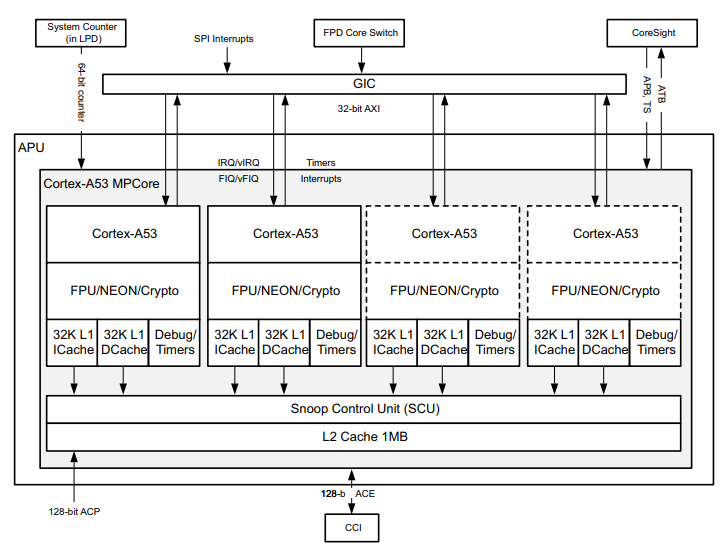
\includegraphics[width=1\textwidth]{./images/apu.jpg}
	\end{center}
	\vspace{-5pt}
	\caption[Detailliertes APU-Blockdiagramm]{Detailliertes APU-Blockdiagramm [\cite{Xilinx2017}[p.~57]]} % Eckige Klammer (optional): Caption-Text in Abbildungsverzeichnis
	\label{fig:zynqmp:apu}
	\vspace{-5pt}
\end{figure}
Andererseits kann ein 128-Bit-Accelerator Coherency Port (ACP) Slave-Controller verwendet werden, wenn ein anderer Block mit Master-Zugriff auf Daten im L2-Cache zugreifen möchte. In der Praxis bedeutet dies, dass der PL auf den L2-Cache über den Port %S_AXI_ACP_FPD zugriffen kann.

\subsubsection{Programmable Logik (PL)}
Dieser Abschnitt bietet einen Überblick über die verfügbaren Funktionen der Zynq Ultrascale+ MPSoC Programmable Logic (PL). Tabelle ~\ref{tab:zcu:vergleich} ist ein Vergleich einiger EG-Bausteine. Es gibt tatsächlich mehr Varianten als die dort aufgeführten. Die FPGA-Fabric besteht hauptsächlich aus Logikzellen und konfigurierbaren Logikblöcken (CLB). Ein CLB kann Flipflops und eine Look-up-Table (LUT) enthalten, muss es aber nicht.\\

\begin{table}[H]
	\centering
	\begin{tabular}{|p{5cm}|p{2cm}|p{2cm}|p{2cm}|}
		\toprule
		\textbf{Gerät Name} & ZU4EV & ZU5EV & ZU7EV \\
		\midrule
		\textbf{System Logic Cells (K)} & 192 & 256 & 504 \\
		\textbf{Speicher (Mb)} & 18.5 & 23.1 & 38.0 \\
		\textbf{DSP-Schnitte} & 728 & 1,248 & 1,728 \\
		\textbf{Video-Code-Einheit (VCU)} & 1 & 1 & 1 \\
		\textbf{Maximale E/A-Pins} & 252 & 252 & 464 \\
		\bottomrule
	\end{tabular}
	\caption[Vergleich einiger Zynq Ultrascale+ MPSoC EG ]{Vergleich einiger Zynq Ultrascale+ MPSoC EG [\cite{XilinxInc.}]}
	\label{tab:zcu:vergleich}
\end{table}

Der Speicher eines FPGAs besteht entweder aus dedizierten Speicherblöcken wie BlockRAM und UltraRAM oder aus CLB, die als RAM-Zellen verwendet werden (Distributed RAM). Schließlich enthält das FPGA eine Reihe von DSP48E2 IP-Blöcken, die Multiplikationen und andere arithmetische/logische Aufgaben effizient durchführen können

\subsection{MCP251XFD CAN Controller + Transceiver}

\begin{figure}[H]
	\begin{center}
		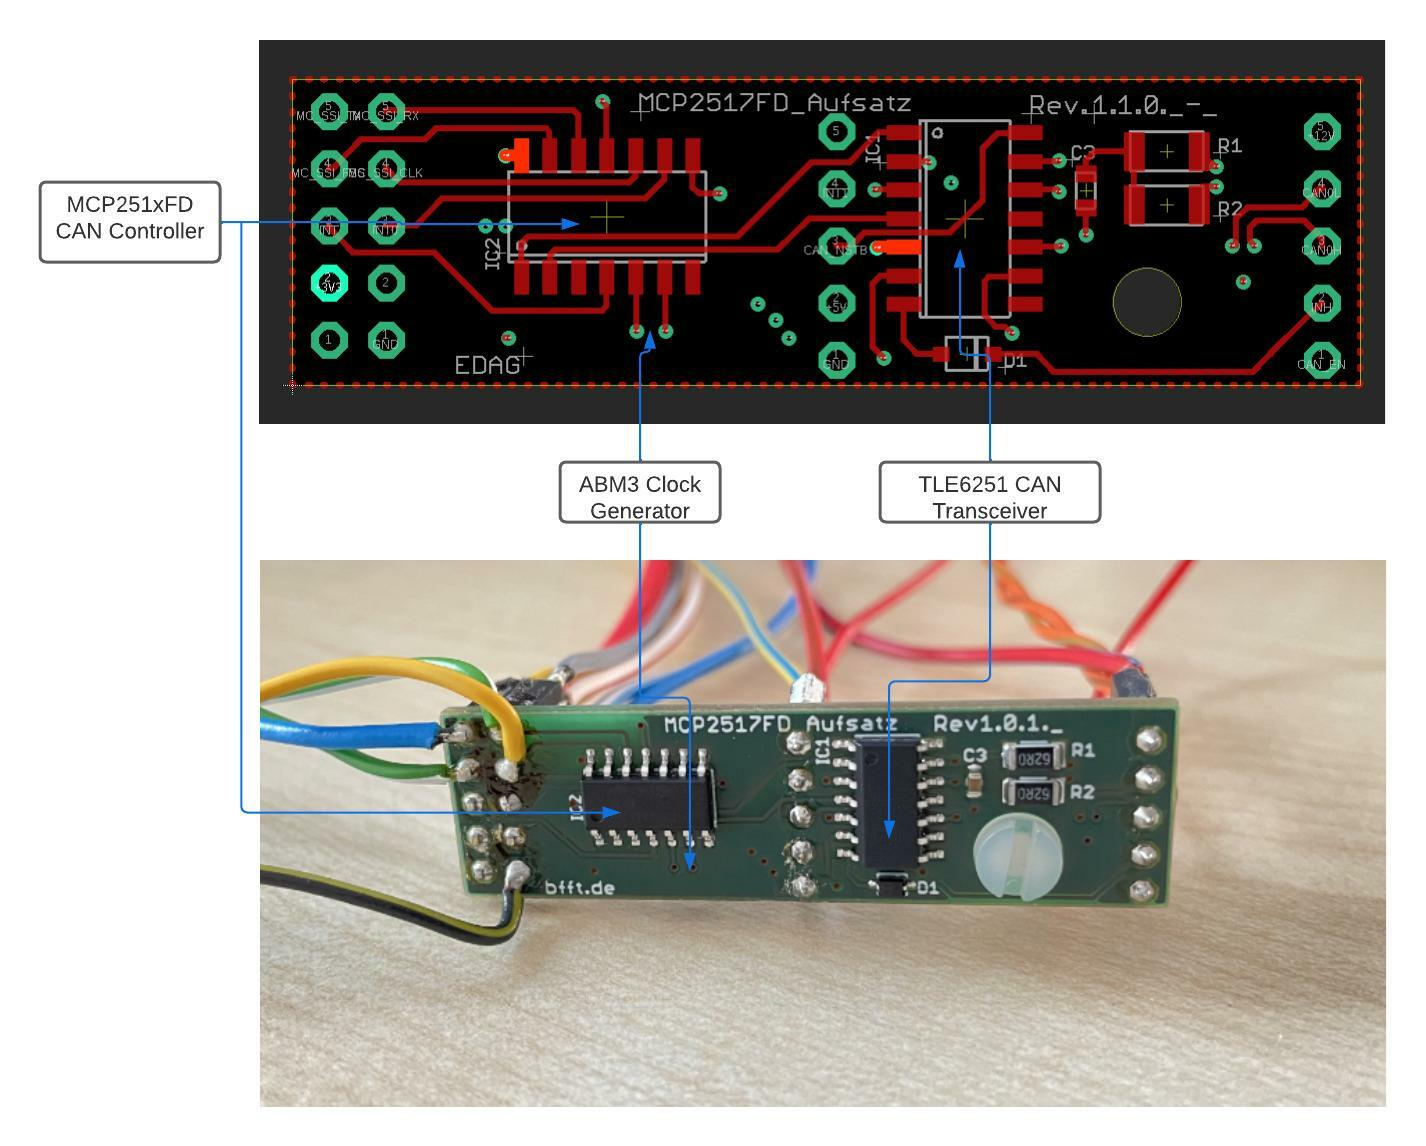
\includegraphics[width=1\textwidth]{./images/mcp_ic_phy.jpg}
	\end{center}
	\vspace{-5pt}
	\caption[CAN-Transceiver- und Controller-Modul]{CAN-Transceiver- und Controller-Modul} % Eckige Klammer (optional): Caption-Text in Abbildungsverzeichnis
	\label{fig:can:controller:transciever}
	\vspace{-5pt}
\end{figure}
Bevor wir uns näher mit diesem CAN-Controller befassen, sollte erklärt werden, dass das \grqq x\grqq\ im Namen des Chips entweder \grqq 7\grqq\ oder \grqq 8\grqq\ werden kann. MCP251XFD unterstützt also MCP2517FD und MCP2518FD.\\
Die Firma entwickelte im Rahmen dieses Projekt, aus kostengünstigen Gründen den  MCP2517FD. Zweck war es, zu prüfen, wie schnell Daten mit diesem CAN-Controller verarbeitet werden können. Auf die Eigenschaften des Chips wird nun im Folgenden eingegangen.\\
Der MCP2517FD-Chip ist ein kompaktes Board, das eine komplette CAN-Lösung bietet und als Steuerknoten in einem CAN-Netzwerk verwendet wird. Wie in Abbildung 1 zu sehen ist, besteht das Board hauptsächlich aus einem CAN-FD-Controller mit SPI-Schnittstelle (MCP2517FD) und einem Hochgeschwindigkeits-CAN-Transceiver (TLE6251). Letzterer stellt eine physikalische Verbindung mit dem CAN-Bus selbst her, während der CAN-Controller MCP2517FD eine Schnittstelle zwischen der MCU und dem PHY darstellt. Die Aufgabe des CAN-Controllers seinerseits ist es, die Arbitrierung, das Nachrichtenframing, die Nachrichtenvalidierung, die Fehlererkennung, die Nachrichtenfilterung und vieles mehr zu übernehmen. Weiterhin unterstützt er sowohl CAN-Frames im klassischen Format (CAN2.0B) als auch im CAN-Flexible-Data-Rate-Format (CAN FD), wie in ISO 11898- 1:2015.\\
Der ISO 11898- 1:2015 hier, der von der International Organization for Standardization (ISO) rausgegeben wurde, spezifiziert das klassische CAN-Rahmenformat und das neu eingeführte CAN Flexible Data Rate Frame Format. Das klassische CAN-Frame-Format erlaubt Bitraten bis zu 1 Mbit/s und Nutzdaten bis zu 8 Byte pro Frame, Das Flexible Data Rate Frame Format erlaubt höhere Bitraten als 1 Mbit/s und Nutzdaten von mehr als 8 Byte pro Frame.

\begin{figure}[H]
	\begin{center}
		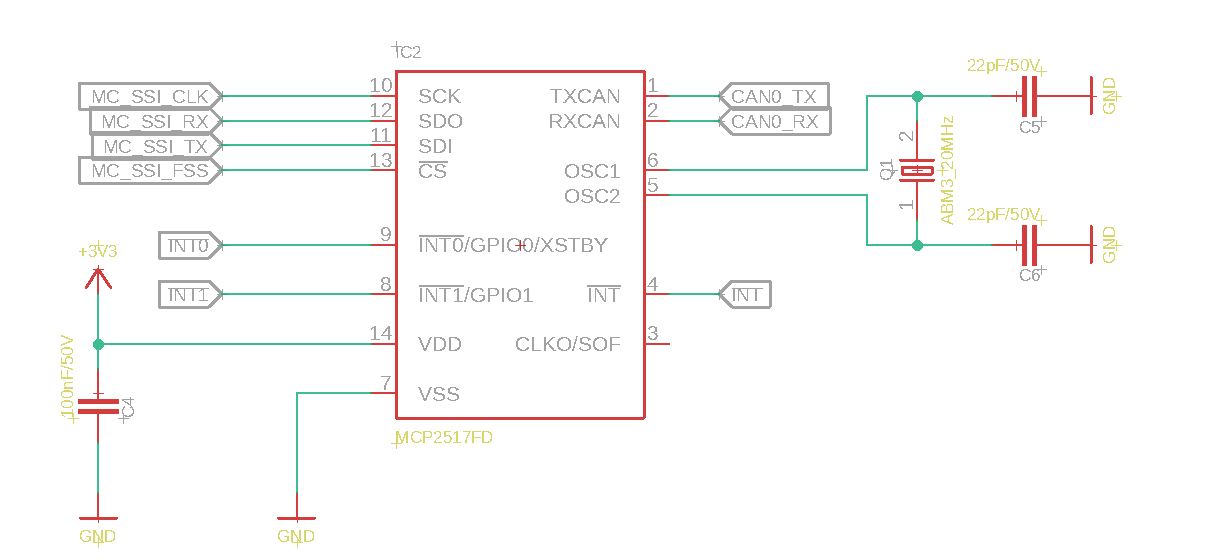
\includegraphics[width=1\textwidth]{./images/mcp_eagle.jpg}
	\end{center}
	\vspace{-5pt}
	\caption[CAN Controller Modul]{CAN Controller Modul} % Eckige Klammer (optional): Caption-Text in Abbildungsverzeichnis
	\label{fig:can:controller}
	\vspace{-5pt}
\end{figure}

Der MCP2517FD enthält die folgenden Hauptblöcke[\cite{Transmission2018}]:
\begin{itemize}
	\item Das CAN FD Controller-Modul implementiert das CAN FD-Protokoll und enthält die FIFOs und Filter.
	\item Die SPI-Schnittstelle, die zur Steuerung des Geräts durch Zugriff auf SFRs und RAM verwendet wird
	\item Der RAM-Controller arbitriert die RAM-Zugriffe zwischen dem SPI- und dem CAN FD Controller-Modul
	\item Der Nachrichten-RAM, der zur Speicherung der Daten der Nachrichtenobjekte verwendet wird
	\item Der Oszillator: Das MCP251XFD CAN Controller verwendet den ABM3 Clock Generator, als Standardtaktquelle für den Chip. Der ABM3 auf diesem Board wurde so programmiert, dass er eine Ausgangsfrequenz von 20 MHz erzeugt.
	
	\begin{table}[H]
		\centering
		\begin{tabular}[h]{|l|c|p{5cm}|}
		%\begin{tabular}{||c|c|p{5cm}||} \hline
			%\toprule
			\hline
			\hline
			\textbf{Pin} & Name & Beschreibung \\
			\hline
			\textbf{1} & CAN0\_TX & TX Interrupt \\
			\hline
			\textbf{2} & CAN0\_RX & RX Interrupt \\
			\hline
			\textbf{3} & CLKO/SOF & \\
			\hline
			\textbf{4} & INT & Interrupt \\
			\hline
			\textbf{5} & OSC1 & Clock Output 1 \\
			\hline
			\textbf{6} & OSC2 & Clock Output 2 \\
			\hline
			\textbf{7} & VSS & Ground \\
			\hline
			\textbf{8} & INT0 &  \\
			\hline
			\textbf{9} & INT1 & \\
			\hline
			\textbf{10} & SCK & SPI Clock \\
			\hline
			\textbf{11} & SDI & SPI Data IN \\
			\hline
			\textbf{12} & SDO & SPI Data OUT \\
			\hline
			\textbf{13} & CS & Chip Select zur Auswahl des Microchips \\
			\hline
			\textbf{14} & VDD & Versorgungsspannung des CAN Module. Die Spapnnung liegt zwischen 3.3V und 5V \\
			\hline
			\hline
		\end{tabular}
		\caption[mcp251xfd Pins]{mcp251xfd Pins}
		\label{tab:mcp:pins}
	\end{table}
	\subsubsection{CAN FD Controller Modul}
	
\end{itemize}

Der Controller kann in verschiedenen Modi eingestellt werden, nämlich
\begin{itemize}
	\item Configuration
	\item Normal CAN FD
	\item Normal CAN 2.0
	\item Sleep
	\item Listen Only
	\item Restricted Operation: Also Eingeschränkter Betrieb
	\item und Internal and External Loop back modes (Interner und externer Loopback-Modus)
\end{itemize}
\subsubsection{TLE6251 CAN Transceiver}
\begin{figure}[H]
	\begin{center}		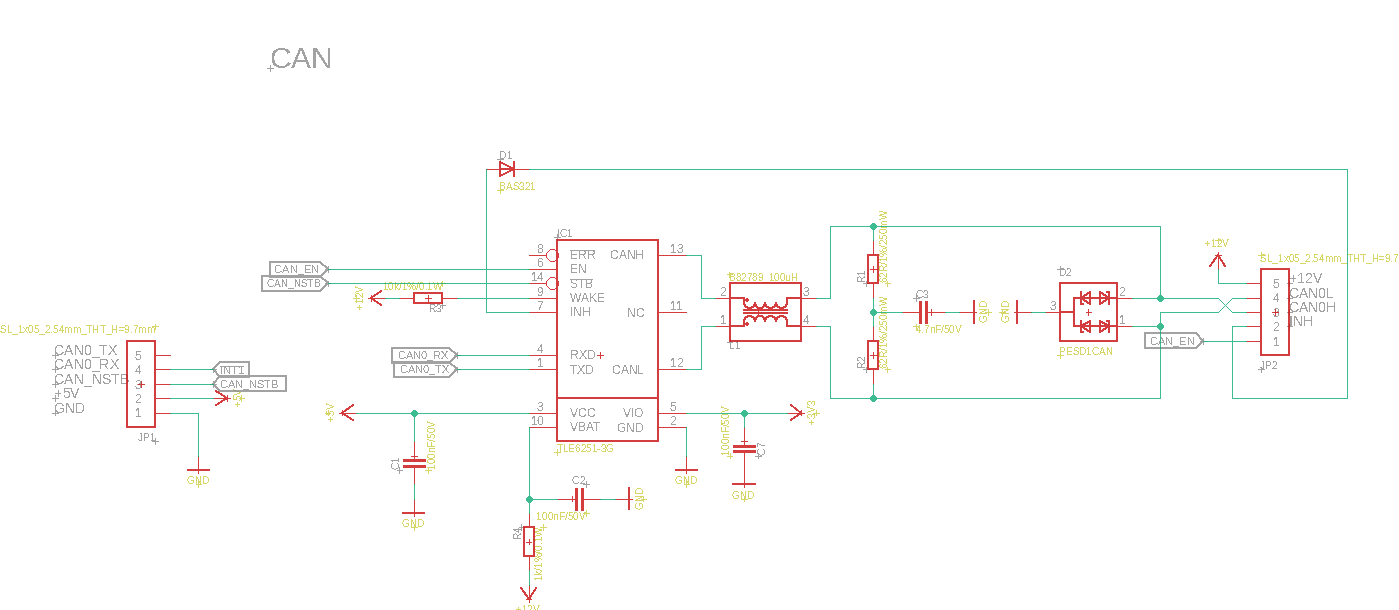
\includegraphics[width=1.2\textwidth]{./images/can_transceiver_eagle.jpg}
	\end{center}
	\vspace{-5pt}
	\caption[CAN Transceiver Modul]{CAN Transceiver Modul} % Eckige Klammer (optional): Caption-Text in Abbildungsverzeichnis
	\label{fig:can:transceiver}
	\vspace{-5pt}
\end{figure}

Der Hochgeschwindigkeits-CAN-Transceiver, der TLE6251, stellt eine physische Verbindung mit dem CAN-Bus her. Dieser ermöglicht eine Kommunikationsgeschwindigkeit von bis zu 5Mbps und unterstützt die Betriebsmodi Normal und Standby. Der Normalmodus ist eingeschaltet, wenn der STBY-Pin, der auf den AN-Pin der mikroBUS geführt wird, auf einem logischen Low-Pegel liegt, während der TXD-Pin auf einem hohen logischen Pegel gehalten wird. Im Normalmodus können die Daten über die CAN H/L-Busleitungen gesendet und empfangen werden.



\section{Konfiguration und Bauen des Systems}
\label{cha:ver:sec:Konfiguration_und bauen_system}
\clearpage

\chapter{Fazit und Ausblick}
\label{cha:Fazit_und_Ausblick}


\section{Fazit}
\label{cha:Fa_und_Aus:sec:Fazit}

Im Rahmen dieser Arbeit \textbf{Konfiguration und Optimierung des Embedded-Linux-Betriebssystem für Automotive Image Processing Unit} wurde den Prozess der Erstellung einer Linux-Distribution für den Zynq UltraScale+ MPSoC bzw. der von Xilinx ZCU106 Baord beschrieben, und illustriert, wie ein  

\section{Ausblick}
\label{cha:Fa_und_Aus:sec:Ausblick}

% Literaturverzeichnis ---------------------------------------------------------
%   Das Literaturverzeichnis wird aus der BibTeX "bibliography.bib" erstellt.
% ------------------------------------------------------------------------------
\bibliography{bibliography} % Aufruf: bibtex Masterarbeit
\bibliographystyle{natdin} %DIN-Stil des Literaturverzeichnisses
%\bibliographystyle{myplainnat} % custom


Ich, \autor, Matrikel-Nr.\ \matrikelnr, versichere hiermit, dass ich die vorliegende Arbeit mit dem Thema
\begin{quote}
\textit{\titel\ - \untertitel}
\end{quote}
selbständig verfasst und keine anderen als die angegebenen Quellen und Hilfsmittel benutzt habe, wobei ich alle wörtlichen und sinngemäßen Zitate als solche gekennzeichnet habe. Die Arbeit wurde bisher keiner anderen Prüfungsbehörde vorgelegt und auch nicht veröffentlicht.\\

\ort, den \today
\vspace*{1cm}\\
\rule[-0.1cm]{5cm}{0.5pt}\\
\textsc{\autor} 
 % Eidesstattliche Erklärung

% Anhang -----------------------------------------------------------------------
%   Die Inhalte des Anhangs werden in der Datei "Anhang.tex" inkludiert.
% ------------------------------------------------------------------------------
\begin{appendix}
    \clearpage
    \pagenumbering{alph}
    \chapter{Anhang}
    \label{sec:Anhang}
    % Rand der Aufzählungen in Tabellen anpassen
    \setdefaultleftmargin{1em}{}{}{}{}{}
    \section{Inhalt des Datenträgers}
\label{apx:Datentraeger}

Der dieser Arbeit beigelegte Datenträger beinhaltet zusätzliche Materialen. 
Neben der Arbeit selbst im Portable Document Format (PDF) befinden sich sowohl die Sources der Implementierungen als auch die lauffähigen Pakete.

\begin{description}
\item[\texttt{./all-my-packages/}] ~ \linebreak 
\noindent\hspace*{10mm} Sources der Packages
\item[\texttt{./Architektur/}] ~ \linebreak 
\noindent\hspace*{10mm} UML-Diagramme der Architektur
\item[\texttt{./Thesis\_Vorname\_Nachname\_123456.pdf}] ~ \linebreak 
\noindent\hspace*{10mm} PDF Version dieser Arbeit
\item[\texttt{./ThesisVM.ova}] ~ \linebreak 
\noindent\hspace*{10mm} Virtual Box Image mit lauffähiger Demoumgebung
\end{description}
\end{appendix}

% Index ------------------------------------------------------------------------
%   Zum Erstellen eines Index, die folgende Zeile auskommentieren.
% ------------------------------------------------------------------------------
%\printindex


\end{document}
